\documentclass[a4paper,11pt,twoside,ngerman,color]{book}
\usepackage[a4paper,left=3.5cm,right=2.5cm,bottom=3.5cm,top=3cm]{geometry}

\usepackage[german,english]{babel}

\usepackage[pdftex]{graphicx,color}
\usepackage{amsmath,amssymb,subfigure}

% Theorem-Umgebungen
\usepackage[amsmath,thmmarks]{ntheorem}

% Korrekte Darstellung der Umlaute
\usepackage[utf8]{inputenc}
\usepackage[T1]{fontenc}

% Codeabschnitte
\usepackage{listings}
\usepackage{lstlinebgrd}

\definecolor{mygreen}{rgb}{0,0.6,0}
\definecolor{mygray}{rgb}{0.5,0.5,0.5}
\definecolor{mymauve}{rgb}{0.78,0,0.72}

\definecolor{design1}{HTML}{639ACE}
\definecolor{design2}{HTML}{53972F}
\definecolor{design3}{HTML}{C33F4F}
\definecolor{design4}{HTML}{DC8C46}
\definecolor{design5}{HTML}{4A34A8}

\lstset{ %
	backgroundcolor=\color{white},   % choose the background color
	basicstyle=\ttfamily\footnotesize,        	 % size of fonts used for the code
	breaklines=true,                 % automatic line breaking only at whitespace
	captionpos=b,                    % sets the caption-position to bottom
	commentstyle=\color{mygreen},    % comment style
	escapeinside={\%*}{*)},          % if you want to add LaTeX within your code
	keywordstyle=\color{blue},       % keyword style
	stringstyle=\color{mymauve},     % string literal style
	frame=single,
	showstringspaces=false,
	tabsize=2,
	numbers=left
}

\lstdefinelanguage{MyC++} {
	language=C++,
	morestring=[s]{/*}{*/},
}

% Bibtex deutsch
\usepackage[backend=biber]{biblatex}
\addbibresource{bibliography.bib}
\renewbibmacro{in:}{%
  \ifentrytype{inbook}{}{\printtext{\bibstring{in}\intitlepunct}}}

% URLs
\usepackage{url}

% Caption Packet
\usepackage[margin=0pt,font=small,labelfont=bf]{caption}

% Zeichnen von Darstellungen
\usepackage{tikz}
\usepackage{pgfplots}
\usepackage{pgfplotstable}

\usetikzlibrary{positioning,calc}

% Hinzufügen weiterer Symbole
\usepackage{bbding}

% Zeilenabstand einstellen %
\renewcommand{\baselinestretch}{1.25}

% Floating-Umgebungen anpassen %
\renewcommand{\topfraction}{0.9}
\renewcommand{\bottomfraction}{0.8}

% Abkürzungen richtig formatieren %
\usepackage{xspace}
\newcommand{\vgl}{vgl.\@\xspace} 
\newcommand{\zB}{z.\nolinebreak[4]\hspace{0.125em}\nolinebreak[4]B.\@\xspace}
\newcommand{\bzw}{bzw.\@\xspace}
\newcommand{\dahe}{d.\nolinebreak[4]\hspace{0.125em}h.\nolinebreak[4]\@\xspace}
\newcommand{\etc}{etc.\@\xspace}
\newcommand{\evtl}{evtl.\@\xspace}
\newcommand{\ggf}{ggf.\@\xspace}
\newcommand{\bzgl}{bzgl.\@\xspace}
\newcommand{\so}{s.\nolinebreak[4]\hspace{0.125em}\nolinebreak[4]o.\@\xspace}
\newcommand{\iA}{i.\nolinebreak[4]\hspace{0.125em}\nolinebreak[4]A.\@\xspace}
\newcommand{\sa}{s.\nolinebreak[4]\hspace{0.125em}\nolinebreak[4]a.\@\xspace}
\newcommand{\su}{s.\nolinebreak[4]\hspace{0.125em}\nolinebreak[4]u.\@\xspace}
\newcommand{\ua}{u.\nolinebreak[4]\hspace{0.125em}\nolinebreak[4]a.\@\xspace}
\newcommand{\og}{o.\nolinebreak[4]\hspace{0.125em}\nolinebreak[4]g.\@\xspace}
\newcommand{\oBdA}{o.\nolinebreak[4]\hspace{0.125em}\nolinebreak[4]B.\nolinebreak[4]\hspace{0.125em}d.\nolinebreak[4]\hspace{0.125em}A.\@\xspace}
\newcommand{\OBdA}{O.\nolinebreak[4]\hspace{0.125em}\nolinebreak[4]B.\nolinebreak[4]\hspace{0.125em}d.\nolinebreak[4]\hspace{0.125em}A.\@\xspace}

% Leere Seite ohne Seitennummer, naechste Seite rechts
\newcommand{\blankpage}{
 \clearpage{\pagestyle{empty}\cleardoublepage}
}

% Keine einzelnen Zeilen beim Anfang eines Abschnitts (Schusterjungen)
\clubpenalty = 10000
% Keine einzelnen Zeilen am Ende eines Abschnitts (Hurenkinder)
\widowpenalty = 10000 \displaywidowpenalty = 10000

% Formatierung von Paragraphen
\setlength{\parskip}{1pt}

% Hyperref-Paket zur Optimierung der PDF
\usepackage{hyperref}

\usepackage[markcase=noupper,headsepline]{scrlayer-scrpage}
\pagestyle{scrheadings}
\clearpairofpagestyles

\setkomafont{pagehead}{\normalfont}

\ohead{\pagemark}
\ihead{\headmark}
\automark[chapter]{chapter}

\hypersetup{
	pdftitle = {Effiziente String-Verarbeitung in Datenbankanfragen auf hochgradig paralleler Hardware},
	pdfauthor = {Florian Lüdiger},
	colorlinks=true,
	allcolors = black
}



\begin{document}
	\selectlanguage{german}
	
	\begin{titlepage}
\definecolor{TUGreen}{rgb}{0.517,0.721,0.094}
\vspace*{-2cm}
\newlength{\links}
\setlength{\links}{-1.5cm}
\sffamily
\hspace*{\links}
\begin{minipage}{12.5cm}

\includegraphics[width=8cm]{bilder/tud_logo_rgb}
%\hspace*{-0.25cm} \textbf{TECHNISCHE UNIVERSIT"AT DORTMUND}\\
%\hspace*{-1.2cm} \rule{5mm}{5mm} \hspace*{0.1cm} FACHBEREICH INFORMATIK\\
\end{minipage}

\vspace*{4cm}

\hspace*{\links}
\hspace*{-0.2cm}
\begin{minipage}{9cm}
\large
\begin{center}
{\Large Diplomarbeit} \\
\vspace*{1cm}
\textbf{Titel der Diplomarbeit} \\
\vspace*{1cm}
Name des Diplomanden\\
% \vspace*{1cm}
Monat der Abgabe
\end{center}
\end{minipage}
\normalsize
\vspace*{5.5cm}

% \hspace*{\links}

\vspace*{2.1cm}

\hspace*{\links}
\begin{minipage}[b]{5cm}
% \normalsize
\raggedright
Gutachter: \\
Name des Erstgutachters \\
Name des Zweitgutachters \\
\end{minipage}

\vspace*{2.5cm}
\hspace*{\links}
\begin{minipage}[b]{8cm}
% \normalsize
\raggedright
Technische Universit"at Dortmund \\
Fakult"at f"ur Informatik\\
Lehrstuhlbezeichnung (LS-Nummer)\\
http://lsXXX-www.cs.tu-dortmund.de
\end{minipage}
%%%%%%%%%%%%%%%%%%%%%%%%%%%%%%%%%%%%%%%%%%%%%%%%%%
% bei Kooperation mit anderen Lehrstuehlen,
% sonst weglassen
\begin{minipage}[b]{8cm}
% \normalsize
\raggedleft
In Kooperation mit:\\
Fakult"atsname\\
Lehrstuhl-/Institutsbezeichnung
\end{minipage}
%%%%%%%%%%%%%%%%%%%%%%%%%%%%%%%%%%%%%%%%%%%%%%%%%%

\end{titlepage}

	\blankpage
	
	\pagenumbering{roman}
	
	\setcounter{tocdepth}{1}
	\tableofcontents
	
	\cleardoublepage
	
	\pagenumbering{arabic}
	
	% Kapitel
	\chapter{Einleitung}

Ein Großteil der Datensätze, die in realen Systemen zum Einsatz kommen enthalten eine große Vielfalt an String-Datensätzen mit verschiedensten Eigenschaften.
Die Operationen, die auf diesen Datensätzen ausgeführt werden reichen von Gleichheitsüberprüfungen über das Enthaltensein eines Teilstrings bis zum Erfüllen eines komplexen, regulären Ausdrucks.
In dieser Arbeit wird untersucht werden, wie sich die unterschiedlichen Operationen zur String-Verarbeitung verhalten, wenn diese auf einer hochgradig parallel arbeitenden Grafikkarte ausgeführt werden.
Außerdem wird analysiert, ob ein Verfahren zur Steigerung der Auslastung der Grafikkarte eine signifikante Leistungssteigerung erzielen kann.

\section{Motivation und Hintergrund}

Die effiziente Berechnung unterschiedlicher Operatoren auf Zeichenketten ist essenziell für das Erreichen eines hohen Durchsatzes und für das Gewährleisten von maximaler Performanz.
In diesem Kontext versprechen Grafikkarten durch ihre hochgradig parallele Architektur in der Theorie eine bestmögliche Leistung.

Der Aufbau von moderner, hoch paralleler Hardware wie einer Grafikkarte führt dazu, dass diese besonders effizient mit gleichmäßigen Daten arbeiten kann.
Ein String-Datensatz ist dagegen typischerweise sehr heterogen durch die unterschiedlichen Längen der einzelnen Zeichenketten, wodurch das Verarbeiten auf einer Grafikkarte zunächst einige Schwierigkeiten birgt.
Aus diesem Grund verwenden bisherige Ansätze zur Verarbeitung von Zeichenketten das Konzept der Dictionaries \cite{Mueller2014}.
Dabei wird eine Tabelle mit allen Strings aufgebaut und zu diesen ein Schlüssel abgespeichert, welcher zusammen mit jedem String in den anderen Tabellen der Datenbank gespeichert wird.
Somit können String-Operationen durch andere Operationen auf den Schlüsseln abgebildet werden, wodurch diese eine einheitliche Struktur und damit ein effizientes Ausführungsmuster auf Grafikkarten erhalten.
Das Aufbauen und Verwalten des für diese Technik verwendeten Dictionaries erzeugt vor allem bei Daten, die sich häufig ändern, einen hohen Aufwand, wodurch die Leistungsfähigkeit des Gesamtsystems sinkt.
Um diesen Verwaltungsaufwand für eine zusätzliche Datenstruktur zu eliminieren, wäre es wünschenswert eine Lösung zu finden, die den Verwaltungsaufwand eliminiert und direkt auf den ursprünglichen String-Daten arbeitet.

Soll eine komplexere Operation auf den Daten ausgeführt werden, die mit regulären Ausdrücken arbeitet, ist die Verwendung eines Dictionaries nicht mehr möglich und spätestens an dieser Stelle muss auf eine andere Methode zurückgegriffen werden.
Die Verwendung von regulären Ausdrücken eröffnet in vielen Anwendungsfällen verschiedenste Möglichkeiten, String-Daten effizient zu verarbeiten und die Leistungsfähigkeiten des Datenbanksystems voll auszunutzen.
Reguläre Ausdrücke stellen ein mächtiges Werkzeug dar, welches den meisten Anwendern von Datenbankmanagementsystemen bekannt ist und vor allem relevant ist, da es das hoch effiziente Auswerten komplexer Muster erlaubt.

Die meisten aktuellen Datenbankmanagementsysteme bieten eine Unterstützung für reguläre Ausdrücke, da sie das effiziente Abgleichen komplexer Muster ermöglichen und dabei eine hohe Leistung garantieren.
Gäbe es eine solche Funktion nicht, müsste eine entsprechende Selektion nach dem Ausführen des Anfrageplans durch das DBMS manuell im Anwendungsprogramm durchgeführt werden.
An dieser Stelle entstehen zahlreiche Probleme, da der Optimierer die Selektion nicht an der optimalen Stelle im Anfrageplan platzieren kann, damit frühzeitig Tupel weg fallen, die nicht in das Ergebnis aufgenommen werden.
Es entsteht also schon beim Datenbankserver eine erhöhte Last durch das unnötige Verarbeiten von Tupeln.
Diese werden zusätzlich noch über das Netzwerk zur Anwendung übertragen, wodurch erneut eine erhöhte Netzlast entsteht.
Die Anwendung wiederum muss anschließend mit einer potenziell geringeren Leistungsfähigkeit als der Datenbankserver die Selektion durchführen, wodurch an dieser Stelle wieder eine unnötig hohe Last entsteht.
Sollten also Anwendungsfälle auftreten, bei denen eine Selektion durch reguläre Ausdrücke gewünscht ist, stellt die Unterstützung dieser Operation durch das Datenbankmanagementsystem einen massiven Vorteil dar.
Auch für Datenbanksysteme, die auf Grafikkarten arbeiten sollte also sichergestellt sein, dass diese die maximal mögliche Performanz bei der Verarbeitung von regulären Ausdrücken erreichen.

\section{Zielsetzung}

In dieser Arbeit sollen verschiedene Operationen, die auf String-Daten arbeiten im Kontext von kompilierten Anfrageplänen mithilfe des Query Compilers DogQC untersucht werden.
Ziel ist es dabei die Performanz der umgesetzten Operatoren zu analysieren und Flaschenhälse, die durch eine schlechte Auslastung der Grafikkarte entstehen, zu identifizieren.
Diese Flaschenhälse sollen mithilfe des Lane Refill-Verfahrens eliminiert werden, wodurch eine Steigerung der Leistungsfähigkeit erreicht werden soll.
Neben einfachen String-Operatoren sollen auch komplexere Techniken, welche reguläre Ausdrücke zur String-Verarbeitung verwenden, analysiert werden und untersucht werden, ob diese einen Laufzeitgewinn durch das Lane Refill erreichen.
Mithilfe dieser Betrachtungen sollen Rückschlüsse darüber gezogen werden, ob das Lane Refill, welches bereits bei der Durchführung von Join-Operationen erfolgreich eingesetzt wird, auch für die Verarbeitung von Zeichenketten einen Nutzen bringt.

\section{Aufbau der Arbeit}

Um verstehen zu können, warum bei der Verarbeitung von String-Daten auf Grafikkarten verschiedene Probleme auftreten können, werden zunächst der Grundaufbau und die wichtigsten Eigenschaften von Grafikprozessoren erklärt.
Anschließend werden die bei DogQC zum Einsatz kommenden Verfahren zur Kompilierung von Anfrageplänen erläutert und die Rahmenbedingungen für die nachfolgenden Untersuchungen festgelegt.
In Kapitel \ref{sec:equals_naiv} wird der einfache String-Vergleich erarbeitet und auf verschiedene Probleme hingewiesen, die im nachfolgenden Kapitel durch den Einsatz des Lane Refill beseitigt werden.
An dieser Stelle wird außerdem erklärt, wie das Lane Refill-Verfahren funktioniert und warum es durch eine höhere Auslastung der Grafikkarte eine bessere Performanz erreichen kann.
Anschließend wird in Kapitel \ref{sec:regex} vorgestellt, wie reguläre Ausdrücke mithilfe von endlichen Automaten ausgewertet werden können und ein geeigneter Ansatz für die Umsetzung im Query Compiler ausgewählt.
Im folgenden Teil wird der parallele Musterabgleich mit regulären Ausdrücken umgesetzt und ähnlich wie beim einfachen String-Vergleich durch das Lane Refill erweitert.
Vorbereitend auf die im letzten Teil der Arbeit durchgeführten Leistungstests der verschiedenen Algorithmen wird aufgezeigt, wie das Optimieren verschiedener Parameter bei der Ausführung von Algorithmen auf einer Grafikkarte einen Einfluss auf die Performanz des Systems nimmt und wie diese Optimierung durchgeführt werden kann.
Schließlich folgen zwei Kapitel zur Evaluation des einfachen String-Vergleichs und des Musterabgleichs mit regulären Ausdrücken, in denen untersucht wird, wie sich die unterschiedlichen Algorithmen verhalten und ob durch die Verwendung des Lane Refill-Verfahrens ein Laufzeitgewinn erreicht werden kann.
Abschließend wird in einem Fazit Stellung dazu genommen, ob die hier beschriebene Zielsetzung erreicht werden konnte und ob das Lane Refill bei der Verarbeitung von Zeichenketten eine sinnvolle Anwendung findet.
	\chapter{Grundlagen der GPU-Programmierung}

Um die in dieser Arbeit vorgestellten Herausforderungen bei der Verarbeitung von String-Daten mit Grafikprozessoren, nachfolgend auch \emph{GPU} genannt, verstehen zu können, ist zunächst ein Verständnis der grundlegenden Eigenschaften aktueller Hardware nötig.
Dabei beschränkt sich diese Untersuchung auf die Grafikkarten-Serie Maxwell von NVIDIA, die hier besprochenen Prinzipien lassen sich allerdings auch auf andere GPUs anderer Hersteller übertragen und finden dort ebenfalls Anwendung.

\section{Grundaufbau einer NVIDIA-Grafikkarte}

Der Hauptprozessor eines Computers, auch \emph{Central Processing Unit (CPU)} genannt, arbeitet eher sequenziell schwerwiegende Threads ab, wodurch individuelle Operationen schnell abgearbeitet werden können, ein hoher Durchsatz allerdings schwierig zu erreichen ist.
Für die Verarbeitung großer Datenmengen wurden daher spezielle Co-Prozessoren in Form von Grafikkarten entwickelt, die hochgradig parallel arbeiten und somit einen massiven Durchsatz erreichen können.
Die \emph{Graphics Processing Unit (GPU)} bildet das Herzstück der Grafikkarte.
Sie besteht aus einer hohen Anzahl an Kernen, die zwar individuell eine vergleichsweise geringe Leistung besitzen, allerdings aufgrund ihrer großen Zahl in datenparallelen Anwendungsfällen in Kombination mit einer hohen Speicherbandbreite eine hervorragende Performanz bieten.

Neben der GPU benötigt eine Grafikkarte noch weitere Peripherie, um effizient funktionieren zu können.
Zur Speicherung der zu verarbeitenden Daten gibt es eigenständige Speichermodule, die unabhängig vom Hauptspeicher des Computers verwaltet werden.
Für die NVIDIA GTX 950, welche im Folgenden als Beispiel genutzt werden soll, beträgt die Größe dieses Speichers 2 GB.
Über eine PCI-Express-Anbindung wird die Kommunikation mit dem Hauptprozessor und die Übertragung der Daten zwischen den Speicherbereichen realisiert.

\begin{figure}[ht]
	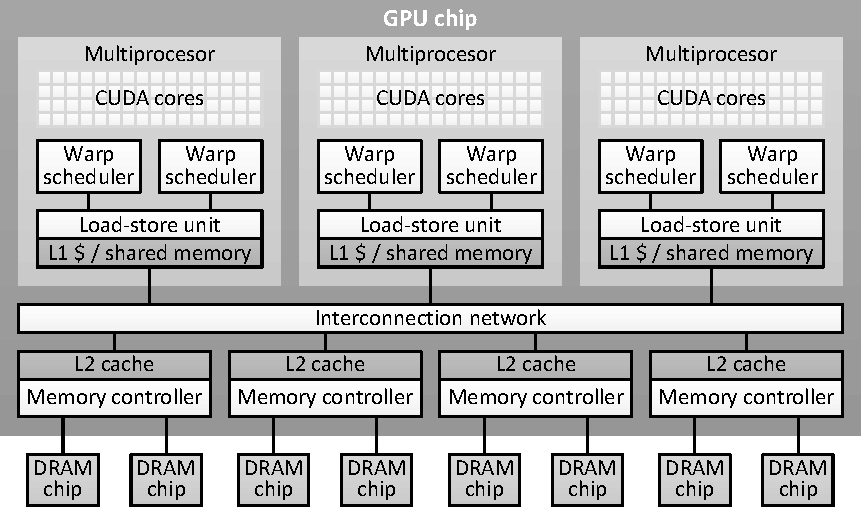
\includegraphics[]{bilder/gpu_architecture.pdf}
	\caption{Architektur einer GPU \cite{Volkov2016}}
	\label{gpu_architecture}
\end{figure}

Wie in Abbildung \ref{gpu_architecture} dargestellt, lässt sich die GPU wiederum in kleinere Module, sogenannte \emph{Streaming Multiprocessors (SM)}, unterteilen, welche jeweils eigenständige Recheneinheiten darstellen.
Eine GT X950 besitzt beispielsweise sechs dieser Streaming Multiprocessors, welche sich ebenfalls in kleinere Einheiten unterteilen lassen.
Die SM bestehen aus vier unabhängigen Blöcken von Rechenkernen, welche jeweils 32 skalare Recheneinheiten, auch \emph{CUDA-Kerne} genannt, beinhalten.
Jeder dieser Blöcke besitzt einen eigenen Scheduler und einige Unterstützungselektronik, sodass diese logisch gesehen ebenfalls unabhängig voneinander arbeiten können. \cite{Nvidia2014}
Bei sechs Streaming Multiprocessors mit jeweils vier Blöcken und 32 Recheneinheiten pro Block besitzt die GT X950 also 768 Kerne, welche über eine Programmierschnittstelle angesprochen werden können.

\section{Scheduling auf GPUs}
\label{sec:cuda_scheduling}

Um die hohe Anzahl von Kernen innerhalb einer GPU effizient mit Arbeit versorgen zu können, ist es wegen des großen Overheads nicht praktikabel, ein individuelles Scheduling für die einzelnen Recheneinheiten durchzuführen.
Aus diesem Grund werden die Threads eines Programms in sogenannte \emph{Warps} zusammengefasst, was damit die kleinste Einheit für das Scheduling bildet.
Ein Warp enthält dabei genau 32 Threads, welche in diesem Kontext auch \emph{Lanes} genannt werden.
Mehrere Warps werden außerdem zu \emph{Blöcken} zusammengefasst, welche schließlich als Ganzes an einzelne Streaming Multiprocessors zugewiesen werden.
Innerhalb eines SM werden Warps ausgetauscht, wenn der vorher aktive Warp beispielsweise auf einen Speicherzugriff wartet, um die dadurch entstehende Latenz zu verstecken.

Über die Anzahl der Threads pro Block und die gesamte Anzahl der Blöcke, ist die Konfiguration des sogenannten \emph{Grids} definiert.
Die Grid-Konfiguration nimmt starken Einfluss auf die Ausführungszeit der Software.
Beispielsweise kann eine zu geringe Anzahl von Threads pro Block dazu führen, dass eventuell entstehende Latenzen nicht mehr so gut versteckt werden können, da nicht genug Threads innerhalb eines SM vorhanden sind.
Eine zu hohe Anzahl von Threads pro Block kann allerdings auch von Nachteil sein, da Hardwareressourcen wie die Speichergröße pro SM gegebenenfalls nicht mehr ausreichen und das Programm nicht mehr korrekt funktioniert.
Das Finden der richtigen Parameter gestaltet sich als äußerst schwierig, da die verwendete Hardware ein komplexes Konstrukt mit vielen Faktoren bildet, die auf Änderungen des Grids Einfluss nehmen.

Eine für die Programmierung von GPUs entscheidende Eigenschaft besteht darin, dass die Threads innerhalb eines Warps parallel ausgeführt werden.
Ähnlich wie bei dem Prinzip \emph{Single Instruction Multiple Data (SIMD)}, führen die Threads in einem Warp die Instruktionen synchron aus, sodass dieses Prinzip auch \emph{Single Instruction Multiple Threads (SIMT)} genannt wird.
Die Trennung in mehrere Threads bietet hierbei den Vorteil, dass eigene Register angesprochen werden können, an unterschiedlichen Stellen im Speicher gelesen werden kann und Threads verschiedene Kontrollflüsse verfolgen können.
Prozesse laufen außerdem zwar logisch parallel ab, allerdings muss dies nicht notwendigerweise physikalisch auch so sein, sodass in einigen Fällen eine höhere Leistung erzielt werden kann.
Für die optimale Performanz einzelner Operationen sollte allerdings gewährleistet sein, dass die Threads größtenteils synchron ausgeführt werden.

Bei der Verwendung von Branching-Instruktionen kann es vorkommen, dass unterschiedliche Threads verschiedene Kontrollflüsse durchlaufen, was auch als \emph{Divergenz} bezeichnet wird.
Da allerdings alle Threads identische Instruktionen ausführen müssen, führt dies dazu, dass sämtliche Threads in einem Warp alle notwendigen Kontrollflüsse durchlaufen und dabei gegebenenfalls das Ergebnis verwerfen, wenn diese sich logisch gesehen in einem anderen Zweig befinden.
Alle Threads, für die der aktuell bearbeitete Kontrollfluss nicht relevant ist, werden als inaktiv bezeichnet.
Inaktive Threads warten somit lediglich auf die aktiven Threads, bis diese die Arbeit innerhalb ihres Kontrollflusses abgeschlossen haben, sodass an dieser Stelle gegebenenfalls massiv Rechenleistung verschwendet wird.
In dieser Problematik liegt der Grund dafür, dass die Verarbeitung von Strings auf Grafikkarten aufgrund ihrer variablen Länge problematisch ist, da die auftretenden Kontrollflüsse divergieren.

\section{Synchronisation von Threads}
\label{sec:synchronisation_von_threads}

Der Compiler und die GPU selbst versuchen innerhalb eines Warps die Anzahl der synchron ausgeführten Operationen zu maximieren, da dadurch eine höhere Leistung erzielt wird \cite{Nickolls2009}.
Diese Synchronisation kann allerdings auch explizit durch den Entwickler erfolgen, indem er die dafür vorgesehenen Operationen der Entwicklungsschnittstelle verwendet.
Das Verwenden solcher Operationen führt dazu, dass alle Threads an dieser Stelle aufeinander warten müssen.

Diese Methoden können außerdem dazu verwendet werden, Informationen über die anderen Threads zu erlangen und die Zusammenarbeit innerhalb der Warps effektiver zu gestalten.
Die Instruktionen werden von der Hardware unterstützt, sodass sie typischerweise sehr effizient ausgeführt werden können.
Ein Beispiel für eine solche Operation ist das Auswerten eines Prädikates für alle Threads und anschließend das Erstellen einer Bitmaske, welche das Ergebnis der Auswertung für alle Threads enthält.
Ein weiteres Beispiel ist das Generieren einer Maske für alle Threads, die in dem aktuellen Ausführungszweig aktiv sind.
Schließlich können noch alle Threads ohne besondere Berechnung synchronisiert werden.
Dies ist zum Beispiel nötig, wenn ein Thread aus dem Speicher lesen will, den andere Threads vorher beschreiben und dieser sicherstellen will, dass die Daten fertig geschrieben wurden \cite{Lin2018}.

\section{Shared Memory}

Eine Kommunikation zwischen Threads innerhalb eines Blocks kann über sogenannten \emph{Shared Memory} geschehen.
Dadurch können größere Mengen von Informationen ausgetauscht werden, als dies über die Synchronisations-Operationen effizient möglich wäre.
Dieser Speicher ist um einige Größenordnungen schneller als der globale Speicher, da sich dieser direkt auf dem Chip der GPU befindet \cite{Harris2013}.
Die Speichergröße innerhalb eines Streaming Multiprocessors ist allerdings beschränkt, weshalb die Anzahl der Threads ebenfalls beschränkt ist, sofern eine große Menge Shared Memory von diesen benötigt wird.

\section{Die CUDA-Programmierschnittstelle für C++}

Für eine effiziente Entwicklung der hochgradig spezialisierten Grafikhardware stellt \mbox{NVIDIA} die \emph{CUDA}-Programmierschnittstelle bereit.
Diese ermöglicht es, die GPU aus einer Hochsprache wie C++ heraus anzusprechen und durch verschiedene Hilfestellungen leicht ein funktionierendes Programm zu erstellen.
Neben vordefinierten Schlüsselwörtern und Syntaxelementen bietet die Entwicklungsumgebung auch einen eigenen Compiler, welcher das erstellte Programm für den Einsatz auf der Grafikkarte optimiert.
Für das Verständnis der Beispiele in dieser Arbeit sollen im Folgenden einige Grundkonzepte des Programmiermodells erläutert werden.

Das Hauptprogramm von CUDA-Programmen besteht aus Code für die CPU, welcher dafür zuständig ist, die Grafikkarte für ihre Aufgabe vorzubereiten und anschließend das Unterprogramm aufzurufen, welches auf der GPU ausgeführt werden soll.
Ein solches Unterprogramm wird \emph{Kernel} genannt und besteht im einfachsten Falle aus einer einfachen Funktion, welche durch das Schlüsselwort \texttt{\_\_global\_\_} gekennzeichnet wird.
In diesem Kontext wird der GPU-Code üblicherweise \emph{Device Code} und der CPU-Code \emph{Host Code} genannt.

Auf die Schnittstellen zur Speicherverwaltung oder zur Festlegung der Grid-Konfiguration aus dem Host Code heraus soll hier nicht weiter eingegangen werden, da für die untersuchten Kriterien lediglich der Device Code interessante Aspekte bietet.

Einem Kernel können verschiedene Parameter wie Zeiger auf Speicherbereiche innerhalb des Grafikspeichers aus dem Hauptprogramm übergeben werden.
Zum Durchlaufen eines solchen Speicherbereiches in einem sequenziellen Programm wäre es ausreichend mit einem Index über das Feld zu iterieren und diesen nach jeder Iteration um eins zu erhöhen.
Bei einer parallelen Architektur würden so allerdings sämtliche Threads über den gesamten Datensatz laufen, anstatt wie gewünscht den Datensatz auf die einzelnen Threads aufzuteilen.
Zu diesem Zweck muss jeder Thread die Informationen darüber haben, welchen globalen Index er innerhalb des Grids hat, um mit dem entsprechenden Element aus dem Datensatz zu beginnen und wie viele Threads in dem Grid vorhanden sind, damit er den entsprechenden Abstand zu dem nächsten zu untersuchenden Element kennt.
Innerhalb eines Kernels kann der Thread auf seinen Threadindex (\texttt{threadIdx.x}), die Anzahl der Threads in einem Block (\texttt{blockDim.x}), seinen Blockindex (\texttt{blockIdx.x}) und die Anzahl der Blöcke im Grid (\texttt{girdDim.x}) zugreifen.
Der globale Index eines Threads berechnet sich somit aus \texttt{blockIdx.x * blockDim.x + threadIdx.x} und die Sprungweite ist definiert durch \texttt{blockDim.x * gridDim.x}.
Die dafür zur Verfügung gestellten Variablen und eine beispielhafte Iteration über zwei Datensätze sind in Listing \ref{cuda_example} dargestellt.

\begin{lstlisting}[language=MyC++,
caption=Beispielhafter CUDA-Kernel zum Iterieren über zwei Datensätze \cite{Harris2017},
label=cuda_example]
__global__
void add(int n, float *x, float *y)
{
	int index = blockIdx.x * blockDim.x + threadIdx.x;
	int stride = blockDim.x * gridDim.x;
	for (int i = index; i < n; i += stride)
		y[i] = x[i] + y[i];
}
\end{lstlisting}

Mit den vorgestellten Informationen zum Grundaufbau von Grafikprozessoren, der Verwaltung von Threads und der Funktionsweise der C++-Programmierschnittstelle werden die in den nachfolgenden Kapiteln vorgestellten Techniken leicht verständlich sein.
	\chapter{Kompilierte Anfragepipelines}
\label{sec:pipelining}

In dieser Arbeit werden String-Vergleiche im Kontext des Query Compilers \emph{DogQC} für GPUs untersucht.
Dieser basiert auf dem Query Compiler \emph{HorseQC} \cite{Funke2018} und wurde für das erleichterte testen von aktuellen Techniken vereinfacht.
DogQC erstellt aus einem gegebenen Anfrageplan mehrere Query Pipelines, die für die Ausführung auf GPUs optimiert sind.
Als Grundlage für die späteren Codebeispiele, wird hier die grundsätzliche Funktionsweise des Query Compilers erklärt und die Vorteile dieser Technik erläutert.

Klassische in-memory Datenbanken wie \emph{MonetDB} arbeiten die Operatoren innerhalb eines Anfrageplans nacheinander ab, was auch \emph{Operator-At-A-Time} genannt wird \cite{Varga2018}.
Dabei wird für den gesamten Datensatz zunächst der erste Operator vollständig ausgeführt, bevor der gesamte Datensatz an den nächsten Operator weiter gegeben wird, bis schließlich der gesamte Anfrageplan abgearbeitet wurde.
Der Nachteil dieser Strategie besteht in einer besonders hohen Lese- und Schreiblast für die Zwischenergebnisse der Operatoren, da diese nach jeder Operation im Speicher materialisiert werden müssen.
Soll die Berechnung auf einer GPU erfolgen, kann es passieren, dass der begrenzte GPU-Speicher nicht ausreicht, um die Zwischenergebnisse zu speichern.
Somit werden während der Berechnung Transfers in den Hauptspeicher des Systems notwendig, um neue Blöcke der Tabelle nachzuladen.
Als Konsequenz entstehen massive Flaschenhälse durch die begrenzte Bandbreite.

\begin{figure}[ht]
	\centering
	\begin{tikzpicture}
		\node (count) {count(*)};
		\node [below = 1cm of count] (join) {$\bowtie$};
		\node [below right = -0.3cm and -0.3cm of join, style={align=center}, font=\linespread{0.7}\selectfont] (join_text) {\scriptsize orders.date=\\ \scriptsize dates.key};
		
		\node [below left = 1cm and 1cm of join] (select_id) {$\sigma$};
		\node [below right = -0.3cm and -0.3cm of select_id] (select_id_text) {\scriptsize year=2019};
		\node [below = 1cm of select_id] (orders) {dates};
		
		\node [below right = 1cm and 1cm of join] (select_year) {$\sigma$};
		\node [below right = -0.3cm and -0.3cm of select_year] (select_year_text) {\scriptsize prio=1};
		\node [below = 1cm of select_year] (dates) {orders};
		
		\draw [thick, shorten > = 0.2cm, shorten < = 0.2cm] (count) -- (join);
		\draw [thick, shorten > = 0.2cm, shorten < = 0.4cm] (join) -- (select_id);
		\draw [thick, shorten > = 0.2cm, shorten < = 0.2cm] (select_id) -- (orders);
		\draw [thick, shorten > = 0.2cm, shorten < = 0.7cm] (join) -- (select_year);
		\draw [thick, shorten > = 0.2cm, shorten < = 0.2cm] (select_year) -- (dates);
		
		\coordinate [below left = 0cm and 0cm of orders] (l1);
		\coordinate [above = 1.7cm of l1] (l2);
		\coordinate [below left = 0.05cm and 0.3cm of join] (l3);
		\coordinate [below left = 0.4cm and 0cm of join] (l4);
		\coordinate [below right = 0cm and 1.3cm of select_id] (l5);
		\coordinate [below right = 0cm and 0cm of orders] (l6);
		
		\draw[thick, dashed, rounded corners=0.2cm]
		(l1) -- (l2) -- (l3) -- (l4) -- (l5) -- (l6) -- cycle;
		
		\coordinate [below left = 0cm and 0cm of dates] (r1);
		\coordinate [above = 1.3cm of r1] (r2);
		\coordinate [above left = -0.1cm and 0.5cm of join] (r3);
		\coordinate [above left = 0cm and 0cm of count] (r4);
		\coordinate [above right = 0cm and 0cm of count] (r5);
		\coordinate [below right = -0.1cm and 1cm of select_year] (r6);
		\coordinate [below right = 0cm and 0cm of dates] (r7);
		
		\draw[thick, dashed, rounded corners=0.2cm]
		(r1) -- (r2) -- (r3) -- (r4) -- (r5) -- (r6) -- (r7) -- cycle;
		
		\node [above left = 1cm and 0cm of select_id] (ht_build) {HT build};
		\coordinate [below left = 0.2cm and 0.6cm of join] (ht_build_arrow_end);
		
		\draw [thick,->] (ht_build) -- (ht_build_arrow_end);
				
	\end{tikzpicture}
	\caption{Beispielplan mit eingezeichneten Pipelines}
	\label{pipeline_example_plan}
\end{figure}

Das Pipelining-Prinzip, welches bei dem vorgestellten Query Compiler zum Einsatz kommt, besagt, dass der Anfrageplan in Pipelines aufgeteilt wird, welche von den Tupeln immer vollständig durchlaufen werden, bevor das Ergebnis materialisiert wird.
Dieses Vorgehen wird \emph{Tuple-At-A-Time} genannt.
Die Operatoren innerhalb des Anfrageplans aus Abbildung \ref{pipeline_example_plan} werden zu zwei Pipelines zusammengefasst.
In der linken Pipeline wird die \textsf{dates}-Relation gelesen, die Selektion ausgeführt und die Hashtabelle für den Join berechnet.
Die rechte Pipeline fasst das Lesen der \textsf{orders}-Relation, die Selektion, die Probe-Operation der Hashtabelle und das Zählen der Ergebnisse zusammen.
Technisch werden die Operationen innerhalb der Pipeline zu einem einzigen Operator verschmolzen, indem der Query Compiler für jede Pipeline einen eigenständigen Kernel generiert, welcher mit der CUDA-Schnittstelle ausgeführt werden kann.
Der Vorteil des Pipelinings besteht drain, dass die Ergebnisse jedes Operators nicht immer wieder im Speicher materialisiert werden müssen, sondern die einzelnen Tupel stets in den GPU-Registern vorgehalten werden können, bis diese fertig verarbeitet wurden.

Klassische \emph{Tuple-At-A-Time}-Ausführungsmuster wie das \emph{Volcano Iterator Model} definieren Operatoren als eigenständige Bausteine mit fest definierten Schnittstellen, die von den Tupeln nacheinander durchlaufen werden \cite{Graefe1994}.
Im Gegensatz dazu werden die Operatoren bei kompilierten Anfragepipelines zu einem Operator verschmolzen, wodurch Funktionsaufrufe entfallen und die Tupel in einem \emph{tight loop} \cite{Neumann2011} verarbeitet werden.

Der Unterschied zwischen kompilierten Anfragepipelines und klassischen \emph{Tuple-At-A-Time}-Ausführungsmustern wie dem \emph{Volcano Iterator Model} liegt darin, dass hier alle , bei dem die einzelnen Operatoren eigenständige Bausteine mit fest definierten Schnittstellen sind, die von den Tupeln nacheinander durchlaufen werden \cite{Graefe1994}.

In Abbildung \ref{pipelining_example_code} wird der Code vorgestellt, welcher von dem Query Compiler für die rechte Pipeline aus dem in Abbildung \ref{pipeline_example_plan} dargestellten Anfrageplan generiert wurde.
Hier ist zu erkennen, dass die drei Operationen innerhalb eines Kernels zusammengefasst wurden, wodurch eine Pipeline entsteht.
Um jedem Thread eine Menge von Tupeln zuweisen zu können, wird zunächst der globale Index des aktuellen Threads innerhalb des Grids berechnet, damit dieser als Schleifenindex \texttt{loop\_var} verwendet werden kann.
Anschließend wird über alle Elemente aus dem Datensatz iteriert, für die der aktuelle Thread zuständig ist.
Die Variable \texttt{active} zeigt im Algorithmus an, ob der aktuelle Thread aktiv läuft oder nur darauf wartet, dass die anderen Threads aus seinem Warp ihre Berechnung abschließen.

In einem Schleifendurchlauf, bei dem das Element mit dem Index \texttt{loop\_var} untersucht wird, wird zunächst die rot markierte Selektion ausgeführt.
Ist diese fehlgeschlagen, da die Priorität der Bestellung nicht bei 1 liegt, wird der Thread deaktiviert und im weiteren Verlauf nicht mehr beachtet, bis er ein neues Tupel erhält.
Hat sich das Tupel qualifiziert, folgt darauf der Hash Probe, welcher in grün dargestellt ist.
Dabei wird das Tupel in der übergebenen Hashtabelle \texttt{hashtable\_date\_key} gesucht und dementsprechend wieder die \texttt{active}-Variable angepasst.
Schließlich wurde vom Query Compiler noch das Zählen der Ergebnisse umgesetzt, welches hier in gelb hervorgehoben wurde.
Dabei wird wieder mithilfe der Synchronisierungsoperation \texttt{\_\_ballot\_sync} die Anzahl der aktiven Lanes gezählt, welche jeweils ein Element des Ergebnisses repräsentieren.
Diese Anzahl wird daraufhin vom ersten Thread innerhalb des Warps auf das Ergebnis addiert. 

Nach der Durchführung der gesamten Pipeline von Operationen für das untersuchte Tupel wird der Index erhöht, sodass im nächsten Schleifendurchlauf das nächste Tupel untersucht wird.
Falls der neu gewählte Index hinter dem Ende der Daten liegt, hat der aktuelle Thread seine Arbeit vollständig abgeschlossen und er wird nicht mehr benötigt, sodass die \texttt{active}-Variable in Zeile 20 auf \texttt{false} gesetzt wird.
Wird anschließend mithilfe der \texttt{\_\_ballot\_sync}-Methode festgestellt, dass sämtliche Lanes inaktiv sind, ist der Datensatz vollständig durchlaufen worden und die Berechnung kann abgeschlossen werden.
Das parallele Abarbeiten eines Warps und das Synchronhalten aller Lanes wird \emph{warp synchronous programming} genannt \cite{Lin2018}.

\begin{figure}[ht]
	\begin{lstlisting}[language=MyC++,
	linebackgroundcolor={%
	\ifnum\value{lstnumber}>24
		\ifnum\value{lstnumber}<28
			\color{red!25}
		\fi
	\fi
	\ifnum\value{lstnumber}>28
		\ifnum\value{lstnumber}<33
			\color{green!25}
		\fi
	\fi
	\ifnum\value{lstnumber}>33
		\ifnum\value{lstnumber}<38
			\color{yellow!25}
		\fi
	\fi
	}]
	__global__
	void joinProbePipeline(
		int *orders_prio,              	// priority attribute of orders table
		int *orders_date,               // date attribute of orders table
		unique_ht *hashtable_date_key,  // hashtable from other pipeline
		int *number_of_matches) {       // return value
		
		// global index of the current thread,
		// used as the iterator in this case
		unsigned loop_var = ((blockIdx.x * blockDim.x) + threadIdx.x);
		
		// offset for the next element to be computed
		unsigned step = (blockDim.x * gridDim.x);
		
		bool active = true;
		bool flush_pipeline = false;
		while(!flush_pipeline) {
		
			// element index must not be higher than number of tuples
			active = loop_var < TUPLE_COUNT_ORDERS;
			
			// break computation when every line is finished and therefore inactive
			flush_pipeline = !__ballot_sync(ALL_LANES, active);
			
			// selection
			if (active)
				active = orders_prio[loop_var] == 1;
			
			// hash join probe
			if (active)
				active = hashProbeUnique(hashtable_date_key, HASHTABLE_SIZE, 
					hash(orders_date[loop_var]))
			
			// count and write
			numProj = __popc(__ballot_sync(ALL_LANES, active))
			if (threadIdx.x % 32 == 0)
				atomicAdd(number_of_matches, numProj);
			
			loop_var += step;
		}
	}
	
	\end{lstlisting}
	\caption{Generierter Kernel für den Beispielplan}
	\label{pipelining_example_code}
\end{figure}

Bei dem hier vorgestellten Verfahren der \emph{Tuple-At-A-Time} Verarbeitung wird klar, dass dieses einen großen Vorteil bei der effizienten Nutzung von schnellem Speicher gegenüber der \emph{Operator-At-A-Time} Verarbeitung bietet.
Zwischenergebnisse müssen nicht mehr materialisiert werden, weshalb Tupel in Registern oder Caches vorgehalten werden können und die Operationen für das explizite Materialisieren entfallen.
Im Gegensatz zu der \emph{Operator-At-A-Time} Technik lässt sich das Pipelining allerdings nicht so einfach auf eine parallele Verarbeitung mit GPUs übertragen.
Wird jedem Thread in einem Warp ein Tupel übergeben, kann es passieren, dass bei beispielsweise einer Selektion dieses Tupel aus der Ergebnisrelation heraus fällt, somit im weiteren Verlauf nicht weiter beachtet werden muss und die entsprechende Lane inaktiv wird.
Dieses Problem wird in Kapitel \ref{sec:unterauslastung_problem} aufgegriffen und in Kapitel \ref{sec:equals_lane_refill} wird ein Lösungsvorschlag dafür vorgestellt.
	\chapter{Einfacher, paralleler String-Vergleich}

Um einige Techniken zur String-Verarbeitung in kompilierten Anfragepipelines auf Grafikkarten entwickeln zu können, wird zunächst ein Operator für den einfachen String-Vergleich für den Query Compiler erarbeitet.
Ein Vergleich auf Gleichheit stellt dabei die einfachste, sinnvolle Variante von String-Verarbeitung dar, wodurch der Einfluss vieler Eigenschaften von Strings auf die Ausführung entsprechender Operationen leicht untersucht werden kann.

Zunächst wird dazu die Motivation hinter einer derartigen Untersuchung erläutert und eine bestehende Technik zur String-Verarbeitung erklärt.
Außerdem wird eine Umsetzung des einfachen String-Vergleichs mittels der CUDA-Schnittstelle ohne spezielle Optimierungen vorgestellt und für einen alternativen Workload für weitere Tests leicht angepasst werden.
Schließlich wird beurteilt, ob die Lösung das Potential hat eine optimale Performanz zu bieten und auf einen Nachteil der einfachen Implementierung eingegangen.

\section{Motivation}

%TODO: todo

\section{Umsetzung des einfachen String-Vergleichs}

Als Basis für die Untersuchungen wird der String-Vergleich-Operator für den Query Compiler zunächst naiv, also ohne tiefgehende Optimierungen umgesetzt.
Mithilfe dieses Operators kann in einer Datenbankabfrage beispielsweise eine Selektion über eine Spalte mit Spring-Daten durchgeführt werden.
Die Anforderung des Operators besteht somit darin, eine Liste von Zeichenketten mit einem vorher spezifizierten String zu vergleichen und zu entscheiden, ob diese identisch sind oder nicht.

Zur Durchführung dieser Operation wird jedem Thread der GPU eine Zeichenkette aus dem Datensatz zugewiesen.
Zunächst wird überprüft, ob die Länge des Strings mit der des Suchstrings übereinstimmt, sodass der entsprechende Eintrag direkt verworfen werden kann.
Sind die Längen identisch, werden beide Zeichenketten Zeichen für Zeichen durchlaufen und diese an jeder Stelle auf Gleichheit überprüft.
Sobald eine Ungleichheit gefunden wurde, wird ein entsprechendes Flag gesetzt und die weiteren Zeichen müssen nicht mehr genauer betrachtet werden.

Sämtliche Threads innerhalb eines Warp werden entsprechend dem Verarbeitungsmodell der GPU parallel abgearbeitet.
Somit sind die Positionen, an denen die Strings verglichen werden ebenfalls für alle Threads identisch.
Sobald der Vergleichsstring im gesamten Warp vollständig durchlaufen wurde, wird das Zwischenergebnis geschrieben.
Sollten alle Threads in dem Warp vorzeitig feststellen, dass keiner der Strings mit dem Suchstring übereinstimmt, wird die aktuelle Untersuchung vorzeitig abgebrochen.

Schließlich wird jedem Thread eine neue Zeichenkette aus dem Datensatz zugewiesen, sodass das Verfahren im weiteren Verlauf wiederholt wird.
Sobald der gesamte Datensatz durchlaufen wurde, ist die Berechnung abgeschlossen.

\tikzset{t_label/.style={rectangle,draw,minimum size=0.4cm,minimum width=2.1cm,inner sep=0pt}}
\tikzset{t_length/.style={rectangle,draw,minimum size=0.4cm,inner sep=0pt,fill=blue!30}}
\tikzset{t_active/.style={rectangle,draw,minimum size=0.4cm,inner sep=0pt}}
\tikzset{t_inactive/.style={rectangle,draw,minimum size=0.4cm,inner sep=0pt,fill=black!30}}
\tikzset{t_blank/.style={rectangle,minimum size=0.4cm,inner sep=0pt}}

\begin{figure}[ht]
	\centering
	\begin{tikzpicture}
	\begin{scope}
	\node (l1) {\textsf{Datensatz:}};
	\node[below = 0cm of l1] (l2) {\textsf{OMA, OPA, OTTO,}};
	\node[below = 0cm of l2] (l3) {\textsf{AHA, OMA, OHM,}};
	\node[below = 0cm of l3] (l4) {\textsf{OHA, DBMS, SQL}};
	\end{scope}
	\begin{scope}[xshift=4cm]
	\node[t_label] (0s) {\textsf{Suchstr.}};
	\node[t_label,below = 0.1cm of 0s] (0a) {\textsf{Thread 1}};
	\node[t_label,below = 0.1cm of 0a] (0b) {\textsf{Thread 2}};
	\node[t_label,below = 0.1cm of 0b] (0c) {\textsf{Thread 3}};
	
	\node[t_length, right = 0.3cm of 0s] (1s) {\textsf{3}};
	\node[t_length, right = 0.3cm of 0a] (1a) {\textsf{3}};
	\node[t_length, right = 0.3cm of 0b] (1b) {\textsf{3}};
	\node[t_length, right = 0.3cm of 0c] (1c) {\textsf{4}};
	
	\node[t_active, right = 0cm of 1s] (2s) {\textsf{O}};
	\node[t_active, right = 0cm of 1a] (2a) {\textsf{O}};
	\node[t_active, right = 0cm of 1b] (2b) {\textsf{O}};
	\node[t_inactive, right = 0cm of 1c] (2c) {};
	
	\node[t_active, right = 0cm of 2s] (3s) {\textsf{M}};
	\node[t_active, right = 0cm of 2a] (3a) {\textsf{M}};
	\node[t_active, right = 0cm of 2b] (3b) {\textsf{P}};
	\node[t_inactive, right = 0cm of 2c] (3c) {};
	
	\node[t_active, right = 0cm of 3s] (4s) {\textsf{A}};
	\node[t_active, right = 0cm of 3a] (4a) {\textsf{A}};
	\node[t_inactive, right = 0cm of 3b] (4b) {};
	\node[t_inactive, right = 0cm of 3c] (4c) {};
	
	\node[t_blank, right = 0cm of 4s] (5s) {};
	\node[t_active, right = 0cm of 4a,fill=green!30] (5a) {\Checkmark};
	\node[t_active, right = 0cm of 4b,fill=red!30] (5b) {\XSolid};
	\node[t_active, right = 0cm of 4c,fill=red!30] (5c) {\XSolid};
	
	\node[t_length, right = 0.1cm of 5s] (6s) {\textsf{3}};
	\node[t_length, right = 0.1cm of 5a] (6a) {\textsf{3}};
	\node[t_length, right = 0.1cm of 5b] (6b) {\textsf{3}};
	\node[t_length, right = 0.1cm of 5c] (6c) {\textsf{3}};
	
	\node[t_active, right = 0cm of 6s] (7s) {\textsf{O}};
	\node[t_active, right = 0cm of 6a] (7a) {\textsf{A}};
	\node[t_active, right = 0cm of 6b] (7b) {\textsf{O}};
	\node[t_active, right = 0cm of 6c] (7c) {\textsf{O}};
	
	\node[t_active, right = 0cm of 7s] (8s) {\textsf{M}};
	\node[t_inactive, right = 0cm of 7a] (8a) {};
	\node[t_active, right = 0cm of 7b] (8b) {\textsf{M}};
	\node[t_active, right = 0cm of 7c] (8c) {\textsf{H}};
	
	\node[t_active, right = 0cm of 8s] (9s) {\textsf{A}};
	\node[t_inactive, right = 0cm of 8a] (9a) {};
	\node[t_active, right = 0cm of 8b] (9b) {\textsf{A}};
	\node[t_inactive, right = 0cm of 8c] (9c) {};
	
	\node[t_blank, right = 0cm of 9s] (10s) {};
	\node[t_active, right = 0cm of 9a,fill=red!30] (10a) {\XSolid};
	\node[t_active, right = 0cm of 9b,fill=green!30] (10b) {\Checkmark};
	\node[t_active, right = 0cm of 9c,fill=red!30] (10c) {\XSolid};
	
	\node[t_length, right = 0.1cm of 10s] (11s) {\textsf{3}};
	\node[t_length, right = 0.1cm of 10a] (11a) {\textsf{3}};
	\node[t_length, right = 0.1cm of 10b] (11b) {\textsf{4}};
	\node[t_length, right = 0.1cm of 10c] (11c) {\textsf{3}};
	
	\node[t_active, right = 0cm of 11s] (12s) {\textsf{O}};
	\node[t_active, right = 0cm of 11a] (12a) {\textsf{O}};
	\node[t_inactive, right = 0cm of 11b] (12b) {};
	\node[t_active, right = 0cm of 11c] (12c) {\textsf{S}};
	
	\node[t_active, right = 0cm of 12s] (13s) {\textsf{M}};
	\node[t_active, right = 0cm of 12a] (13a) {\textsf{H}};
	\node[t_inactive, right = 0cm of 12b] (13b) {};
	\node[t_inactive, right = 0cm of 12c] (13c) {};
	
	\node[t_blank, right = 0cm of 13s] (14s) {};
	\node[t_active, right = 0cm of 13a,fill=red!30] (14a) {\XSolid};
	\node[t_active, right = 0cm of 13b,fill=red!30] (14b) {\XSolid};
	\node[t_active, right = 0cm of 13c,fill=red!30] (14c) {\XSolid};
	
	\node[above = 0.1cm of 1s] (arr1) {};
	\node[above = 0.1cm of 14s] (arr2) {};
	\draw[->, thick] (arr1) -- (arr2) node[midway, above] {{\large\textsf{Ausführungszeit}}};
	\end{scope}
	
	\begin{scope}
	\node[below = 0.5cm of 1c] (laenge) {\textsf{Längenvergleich}};
	\node[below = -0.2cm of 1c] (laenge_arrow) {};
	\draw [->] (laenge) -- (laenge_arrow);
	
	\node[below right = -0.2cm and -0.08cm of 5c] (neue_daten_arrow) {};
	\node[below = 1.3cm of neue_daten_arrow, align = center] (neue_daten) {\textsf{Ergebnis schreiben,} \\ \textsf{neue Daten laden}};
	\draw [->] (neue_daten) -- (neue_daten_arrow);
	
	\node[below = 0.5cm of 14c] (abbruch) {\textsf{frühzeitiger Abbruch}};
	\node[below = -0.2cm of 14c] (abbruch_arrow) {};
	\draw [->] (abbruch) -- (abbruch_arrow);
	\end{scope}
	\end{tikzpicture}
	\caption{Funktionsweise des Algorithmus innerhalb eines Warps mit drei Threads}
	\label{equals_naiv_algorithmus}
\end{figure}

In Abbildung \ref{equals_naiv_algorithmus} ist der Ablauf des Algorithmus innerhalb eines Warps mit drei Threads dargestellt.
Es ist erkennbar, an welchen Stellen die Lanes inaktiv werden, wann die Berechnung frühzeitig abgebrochen werden kann und an welchen Stellen das Ergebnis geschrieben wird und neue Daten aus dem Datensatz geholt werden.

\begin{lstlisting}[language=C++,
	caption=Naive Implementierung einer Selektion von Strings,
	label=naive_equals]
data_length = char_offset[loop_var+1] - char_offset[loop_var] - 1;

// if string lengths are unequals, discard
if (active && data_length != search_length)
	active = false;

int search_id = 0;

// iterate over strings completely or until they don't match anymore
while(active && search_id < search_length) {
	int data_id = search_id + char_offset[loop_var];
	
	// when strings don't match, inactivate the lane
	if (active && data_content[data_id] != search_string[search_id])
		active = false;
	
	search_id++;
}
\end{lstlisting}

In Listing \ref{naive_equals} ist die Implementierung des Operators dargestellt, welcher in einer kompilierten Anfragepipeline die Selektion eines String-Attributs durchführen kann.
Dieser würde beispielsweise die rot markierte Selektion in Listing \ref{pipelining_example_code} ersetzen, falls das \emph{prio}-Attribut in dem Beispiel aus Abbildung \ref{pipeline_example_plan} Strings enthalten würde und alle Bestellungen mit der Priorität \emph{HIGH} gesucht werden würden.
Nach Abschluss der Berechnung ist der Wert der \texttt{active}-Variable genau dann \texttt{true}, wenn der String mit dem gesuchten String übereinstimmt, sodass im Anschluss mit weiteren Operationen fortgefahren werden kann.

Diese Implementierung erwartet, dass einige Daten vorher vom Hauptspeicher in den Speicherbereich der GPU kopiert wurden und dort zur Verfügung stehen.
Der Datensatz, der mit dem Vergleichsstring abgeglichen werden soll, besteht aus einer Aneinanderreihung der entsprechenden Zeichenketten ohne Trennzeichen und ist in der Variable \texttt{data\_content} gespeichert.
Damit daraus die ursprünglichen Strings extrahiert werden können, gibt es das Feld \texttt{char\_offset}, welches Informationen über die Indizes der Einzelstrings innerhalb des Datensatzes enthält.
Ebenfalls muss natürlich ein Zeiger auf den Suchstring und dessen Länge in den entsprechenden Parametern \texttt{search\_string} und \texttt{search\_string\_length} vorhanden sein.
Um die Berechnung rechtzeitig vor Speicherüberschreitungen abbrechen zu können, wird schließlich noch die Variable \texttt{line\_count} benötigt, welche die Anzahl der Zeichenketten im Datensatz beschreibt.

Im ersten Schritt wird für einen String überprüft, ob dessen Länge mit der des Suchstrings übereinstimmt und dieser anderenfalls verworfen.
Sind die Längen identisch, wird in der Schleife über beide Zeichenketten iteriert, bis das Ende beider erreicht wurde, oder festgestellt wird, dass ein Zeichen aus dem Vergleichsstring nicht mit dem aus dem Suchstring übereinstimmt.
An dieser Stelle fällt die parallele Struktur des Kernels besonders auf, da die Zeichen aller Strings parallel von den Threads durchlaufen werden und diese erst aufhören, wenn der letzte Thread den ihm zugewiesenen Datensatz vollständig durchlaufen hat.
Ist die Schleife abgeschlossen oder vorzeitig abgebrochen worden, kann am Zustand der \texttt{active}-Variable abgelesen werden, ob die Strings übereinstimmen oder nicht.

\section{Präfixtest als alternativer Workload}

\section{Schlechte Auslastung der GPU}

	\chapter{Verbesserung des einfachen String-Vergleichs}
\label{sec:equals_lane_refill}

Zur Verbesserung der Auslastung der GPU bei der Berechnung des einfachen String-Vergleichs, wird ein Verfahren vorgestellt, das auch im Kontext der kompilierten Anfragepipelines eine optimierte Laufzeit verspricht.
Dieses stellt durch Verwendung eines Puffers sicher, dass zu jeder Zeit während der Laufzeit die Auslastung eines Warps über einem bestimmten Grenzwert liegt.
Das Prinzip wurde im Kontext von kompilierten Anfragepipelines mit SIMD als \emph{consume everything} vorgestellt \cite{Lang2018} und im Kontext dieser Arbeit auf Grafikkarten angewendet.
Im Folgenden wird das Verfahren als \emph{Lane Refill} bezeichnet, da es die inaktiven Lanes in einem Warp dynamisch wieder auffüllt.

\section{Funktionsweise des String-Vergleichs mit Lane Refill}

Zur Verbesserung des einfachen String-Vergleichs, kann das naive Verfahren durch das Lane Refill erweitert werden, indem ein Puffer eingeführt wird, in dem teilweise abgearbeitete Tupel zwischengespeichert werden können.
Bei der ursprünglichen Technik gibt es drei Stellen, an denen Lanes innerhalb eines Warps inaktiv werden können.
Zum einen passiert dies, wenn beim Längenvergleich zu Beginn eine unpassende Länge festgestellt wird und zum anderen wenn beim Vergleich von zwei Zeichen ein Unterschied festgestellt wird.
Schließlich werden Lanes ebenfalls inaktiv, wenn diese ihren Vergleich abgeschlossen haben und einen passenden String gefunden haben.
Jeweils nach diesen Ereignissen soll nun überprüft werden, ob die Auslastung des Warps noch ausreichend ist, um den Grenzwert zu erreichen.
Ist dieser Grenzwert unterschritten, können wiederum zwei Fälle auftreten.
Sollten sich im Puffer noch ausreichend Tupel befinden, sodass durch Auffüllen der Grenzwert wieder erreicht ist, so werden die inaktiv gewordenen Lanes mit den Zeichenketten aus den gepufferten Tupeln befüllt und es wird weiter gerechnet.
Wurden zuvor zu wenige Elemente gepuffert, sodass der Grenzwert nicht erreicht werden kann, werden die Tupel aus den aktiven Lanes im Puffer gespeichert und die Pipeline mit frischen Tupeln neu gestartet, damit später neue Zeichenketten für den String-Vergleich bereitstehen.

\begin{figure}[ht]
	\centering
	\begin{tikzpicture}
	\node (x11) [draw,thick,minimum width=3,minimum height=3] {};
	\node (x12) [draw,thick,minimum width=3,minimum height=3, right = 0.5cm of x11] {};
	\node (x13) [draw,thick,minimum width=3,minimum height=3, right = 0.5cm of x12] {};
	\node (x14) [draw,thick,minimum width=3,minimum height=3, right = 0.5cm of x13] {};
	\node (x21) [draw,thick,minimum width=3,minimum height=3, below = 0.5cm of x11] {};
	\node (x22) [densely dashed, draw,thick,minimum width=3,minimum height=3, right = 0.5cm of x21] {};
	\node (x23) [draw,thick,minimum width=3,minimum height=3, right = 0.5cm of x22] {};
	\node (x24) [draw,thick,minimum width=3,minimum height=3, right = 0.5cm of x23] {};
	\node (x31) [densely dashed, draw,thick,minimum width=3,minimum height=3, below = 0.5cm of x21] {};
	\node (x32) [densely dashed, draw,thick,minimum width=3,minimum height=3, right = 0.5cm of x31] {};
	\node (x33) [draw,thick,minimum width=3,minimum height=3, right = 0.5cm of x32] {};
	\node (x34) [draw,thick,minimum width=3,minimum height=3, right = 0.5cm of x33] {};
	
	\node (x41) [draw,thick,minimum width=1,minimum height=1, below = 0.8cm of x31] {};
	\node (x42) [draw,thick,minimum width=3,minimum height=3, right = 0.5cm of x41] {};
	\node (x43) [draw,thick,minimum width=3,minimum height=3, right = 0.5cm of x42] {};
	\node (x44) [draw,thick,minimum width=3,minimum height=3, right = 0.5cm of x43] {};
	
	%buffer tuples
	\node (xb1) [draw,thick,minimum width=3,minimum height=3, right = 0.8cm of x44] {};
	\node (xb2) [draw,thick,minimum width=3,minimum height=3, below = 0.5cm of xb1] {};
	\node (xb3) [rotate=-90, below right = 0cm and 0.05cm of xb2] {\footnotesize $\cdots$};
	
	%buffer
	\node (rect) [draw, thick, minimum width = 0.7cm, minimum height = 2cm, below right = -0.7cm of xb1] {};
	\node[align=center, font=\footnotesize, rotate=-90, above right = 0.25cm and 0cm of rect] (b) {\textsf{divergence buffer}};
	
	%flush
	\coordinate [below = 0.2cm of x33] (fl1);
	\coordinate [below = 0.2cm of x34] (fl2);
	\coordinate [above = 0.38cm of rect] (fl3);
	
	\draw[->, thick] (x33) -- (fl1) -- (fl3) -- (rect);
	\draw[thick] (x34) -- (fl2);
	\node[align=center, font=\footnotesize, above left = 0cm of fl3] (b) {\textsf{flush}};
	
	%new elements
	\coordinate [above = 0.2cm of x41] (ne1);
	\coordinate [above = 0.2cm of x42] (ne2);
	\coordinate [above = 0.2cm of x43] (ne3);
	\coordinate [above = 0.2cm of x44] (ne4);
	\coordinate [left = 0.4cm of ne1] (ne5);
	
	
	\node (new) [above right = 0cm and -0.5cm of ne1] {\footnotesize \textsf{new elements}};
	\draw[->, thick] (ne1) -- (x41);
	\draw[->, thick] (ne2) -- (x42);
	\draw[->, thick] (ne3) -- (x43);
	\draw[->, thick] (ne5) -- (ne4) -- (x44);
	
	\node (x51) [densely dashed, draw,thick,minimum width=3,minimum height=3, below = 0.5cm of x41] {};
	\node (x52) [draw,thick,minimum width=3,minimum height=3, right = 0.5cm of x51] {};
	\node (x53) [draw,thick,minimum width=3,minimum height=3, right = 0.5cm of x52] {};
	\node (x54) [draw,thick,minimum width=3,minimum height=3, right = 0.5cm of x53] {};
	
	\node (x61) [densely dashed, draw,thick,minimum width=3,minimum height=3, below = 0.5cm of x51] {};
	\node (x62) [draw,thick,minimum width=3,minimum height=3, right = 0.5cm of x61] {};
	\node (x63) [draw,thick,minimum width=3,minimum height=3, right = 0.5cm of x62] {};
	\node (x64) [densely dashed, draw,thick,minimum width=3,minimum height=3, right = 0.5cm of x63] {};
	
	%refill 
	\coordinate [below = 0.2cm of x61] (rf1);
	\coordinate [below = 0.2cm of x64] (rf2);
	\coordinate [below = 0.23cm of rect] (rf3);
	\draw[->, thick] (rect) -- (rf3) -- (rf1) -- (x61);
	\draw[->, thick] (rf2) -- (x64);
	\node[align=center, font=\footnotesize, below left = 0cm of rf3] (b) {\textsf{refill}};
	
	\node (x71) [draw,thick,minimum width=3,minimum height=3, below = 0.5cm of x61] {};
	\node (x72) [draw,thick,minimum width=3,minimum height=3, right = 0.5cm of x71] {};
	\node (x73) [draw,thick,minimum width=3,minimum height=3, right = 0.5cm of x72] {};
	\node (x74) [draw,thick,minimum width=3,minimum height=3, right = 0.5cm of x73] {};
	
	\node[rotate=-90, below right = 0.2cm and 0.5cm of x72] (xend) {\LARGE $\cdots$};
	\node (ts) [left = 0.5cm of x11] {};
	\node (te) [left = 0.5cm of x71] {};
	\draw[->, thick] (ts) -- (te);
	\end{tikzpicture}
	\caption{Funktionsweise des Lane Refill (Quelle: Henning Funke)}
	\label{fig:divergence_buffer}
\end{figure}

In Abbildung \ref{fig:divergence_buffer} ist die Funktionsweise der vorgestellten Technik dargestellt.
Es ist zu erkennen, dass aktive Tupel in einem schlecht ausgelasteten Warp im Puffer zwischengespeichert werden, was hier als \emph{flush} bezeichnet wird.
Im Anschluss fließen neue Tupel über den Weg der Pipeline wieder in den Warp ein, wodurch dieser wieder vollständig ausgelastet ist.
Sobald erneut eine Unterauslastung auftritt, werden die zwischengespeicherten Elemente aus dem Puffer in die inaktiven Lanes geladen und der Warp ist wieder komplett ausgelastet.

\section{Struktur des optimierten String-Vergleichs im Kernel}

Um den einfachen String-Vergleich durch Lane Refill zu optimieren, muss die Struktur des Operators im Kernel etwas angepasst werden, was in Listing \ref{equals_lane_refill_code} dargestellt wird.
Die äußere Schleife ist bereits aus der Grundstruktur einer Pipeline, wie sie in Kapitel \ref{sec:pipelining} vorgestellt wurde, bekannt und wurde hier für ein leichteres Verständnis aufgegriffen.
Innerhalb der Schleife werden wie bei der naiven Implementierung zunächst die Operatoren ausgeführt, die in der Pipeline vor dem String-Vergleich stehen und es wird die Länge der Zeichenkette untersucht und diese gegebenenfalls verworfen.

Um im nächsten Schritt beurteilen zu können, ob eine ausreichende Auslastung besteht, wird zunächst mithilfe einer Synchronisierungsoperation überprüft, wie viele Lanes im Warp aktiv sind.
Sind im Puffer und im Warp im Summe noch ausreichend aktive Elemente vorhanden, um den vorher definierten Grenzwert zu überschreiten, so kann weiter mit dem String-Vergleich fortgefahren werden.
Gegebenenfalls werden zuvor allerdings noch die leeren Lanes mit Tupeln aus dem Puffer wieder aufgefüllt, sollten die aktiven Lanes alleine nicht ausreichen, um den Grenzwert zu erreichen.
Der eigentliche Vergleich zweier Zeichen funktioniert hier wieder genau wie bei der naiven Implementierung.
Nach dem Vergleich wird geprüft, ob der String vollständig durchlaufen wurde und entsprechend die folgenden Operationen in der Pipeline ausgeführt.
An dieser Stelle fällt auf, dass im Gegensatz zu der naiven Implementierung eine Verschachtelung entsteht, da die Folgeoperationen innerhalb der \texttt{while}-Schleife des String-Vergleichs-Operators ausgeführt werden.

Ist nach erneuter Zählung der aktiven Lanes die Schleifenbedinugng nicht mehr erfüllt, da zu wenige Tupel existieren, um eine ausreichende Auslastung zu gewährleisten, werden die Tupel aus den restlichen, aktiven Lanes in den Puffer geschrieben.
Schließlich wird die Pipeline mit frischen Tupeln wieder von vorne gestartet.

\newpage

\begin{lstlisting}[language=C++,
caption=Struktur der String-Selektion mit Lane Refill,
label=equals_lane_refill_code]
while(!flush_pipeline) {

	/* execute previous operators in the pipeline */
	
	// if string lengths are unequal, discard
	if (active && data_length != search_length)
		active = false;
	
	int numactive = __popc(__ballot_sync(ALL_LANES, active));
	int bufferelements = 0;
	
	while(bufferelements + numactive > THRESHOLD) {
	
		if (numactive < THRESHOLD) {
		
			/* refill empty lanes from buffer in case of underutilization */
			
			bufferelements = bufferelements - numrefill;
		}
		
		// when strings don't match, inactivate the lane
		if (active && data_content[data_id] != search_string[search_id])
			active = false;
		
		search_id++;
		
		if (search_id == search_length) {
		
			/* execute following operators in the pipeline */
		
		}
		
		numactive = __popc(__ballot_sync(ALL_LANES, active));
	}
		
	if (numactive > 0) {
	
		/* flush active lanes to buffer */
		
		bufferelements += numactive;
		active = false;
	}
	
	loop_var += step;
}
\end{lstlisting}

\section{Technische Umsetzung der Pufferung}

Der Puffer wird mithilfe der CUDA-Programmierschnittstelle als Shared Memory umgesetzt, um eine effiziente Kommunikation zwischen den Lanes zu ermöglichen.
Für den einfachen String-Vergleich werden dazu zwei Speicherbereiche benötigt, welche mit dem Schlüsselwort \texttt{\_\_shared\_\_} initialisiert werden.
In einem Feld wird die Position des untersuchten Strings gespeichert und in dem anderen Feld wird der Index des Zeichens innerhalb des Strings gespeichert, das als nächstes verglichen werden muss.
Da der Shared Memory immer auf dem Level eines ganzen Blocks gültig ist, muss dieser so viele Elemente fassen können wie es Threads pro Block gibt.
Eine ausführliche Version der Umsetzung befindet sich in Anhang \ref{apx:equals_lane_refill}, hier sollen aber dennoch die Techniken zum Zwischenspeichern und Laden von Elementen kurz beschrieben werden.

\begin{lstlisting}[language=C++,
caption=Befüllen inaktiver Lanes mit Elementen aus dem Puffer,
label=refill_code]
if (numactive < THRESHOLD) {
	numRefill = min(32 - numactive, bufferelements);
	numRemaining = bufferelements - numRefill;
	
	previous_inactive = __popc(~__ballot_sync(ALL_LANES, active) & prefixlanes);
	
	if (!active && previous_inactive < bufferelements) {
		buf_ix = numRemaining + previous_inactive + bufferbase;
		search_id = search_id_divergence_buffer[buf_ix];
		current = current_divergence_buffer[buf_ix];
		active = true;
	}
	
	bufferelements -= numRefill;
}
\end{lstlisting}

Bei dem in Listing \ref{refill_code} dargestellten Befüllen von leer gelaufenen Lanes mit Elementen aus dem Puffer, bleiben die noch aktiven Lanes unberührt.
Die inaktiven Lanes müssen zunächst beurteilen, ob diese berechtigt sind, sich ein Tupel aus dem Puffer zuzuweisen.
Befinden sich beispielsweise zwei Elemente im Puffer, es gibt aber drei inaktive Lanes, dann erhalten die zwei Lanes mit dem niedrigeren Index ein neues Tupel und die Lane mit höherem Index bleibt weiter inaktiv.
Als erstes muss also bestimmt werden, wie viele Lanes vor der betrachteten Lane inaktiv sind.
Der Wert \texttt{prefixlanes} ist dabei eine Bitmaske mit einem Bit für jede Lane im Warp, bei der für alle vor der aktuellen Lane liegenden Lanes ein Bit gesetzt wurde.
Gibt es weniger inaktive Lanes vor der betrachteten als Elemente im Puffer, darf sich diese Lane ein neues Tupel aus dem Puffer holen.

%TODO: Abbildung einfügen

Um das richtige Element zu erhalten, muss zunächst wie in Abbildung RRRRRRRRRRRRRREFERENZZZZZZZZZZZZZZZZZ dargestellt dessen Index im Puffer errechnet werden, welcher sich aus verschiedenen Offsets Zusammensetzt.
\texttt{buffer\_base} bestimmt dabei die Position des Speicherbereichs, welcher dem aktuellen Warp im Block zugewiesen wurde.
Da der Puffer grundsätzlich von rechts abgearbeitet wird, muss noch der Wert \texttt{num\_remaining} für die Elemente, die im Puffer verbleiben sollen, addiert werden und schließlich noch die Tupel übersprungen werden, die für Lanes mit niedrigerem Index bestimmt sind.

Ist der Index berechnet, können der String und der Suchindex innerhalb des Strings aus dem Puffer geladen werden und die Lane wieder aktiv geschaltet werden.

\begin{lstlisting}[language=C++,
caption={Auslagern übriger, aktiver Lanes in den Puffer},
label=flush_code]
if (numactive > 0) {
	previous_active = __popc(__ballot_sync(ALL_LANES, active) & prefixlanes);
	buf_ix = bufferbase + bufferelements + previous_active;
	
	if(active) {
		search_id_divergence_buffer[buf_ix] = character_index;
		current_divergence_buffer[buf_ix] = current;
	}
	
	bufferelements += numactive;
	active = false;
}
\end{lstlisting}

Das in Listing \ref{flush_code} dargestellte Verfahren zum Einlagern übriger, aktiver Lanes in den Puffer funktioniert ähnlich wie das wieder befüllen von Lanes.
Zunächst wird wieder der Index berechnet, auf den die aktuelle Lane im Puffer zugreifen kann, was identisch zu dem in Abbildung RRRRRRRREFERENZZZZZZZZ dargestellten Verfahren funktioniert, nur dass in diesem Falle die aktiven Lanes statt der inaktiven Lanes als Offset verwendet werden.
Alle verbleibenden, aktiven Lanes speichern daraufhin die Position ihres vorher untersuchten Strings und den als nächstes zu untersuchenden Index innerhalb des Strings im Puffer ab.
Schließlich wird noch die Anzahl der Elemente im Puffer erhöht und der Algorithmus kann anschließend wie gehabt verfahren.

\section{Reduzierung des Overheads}

Ein Nachteil dieses Verfahrens liegt darin, dass durch das Verwalten des Puffers ein erhöhter Overhead entsteht, der die bessere Performanz durch eine gute Auslastung der GPU überschatten könnte.
Um diesen Overhead zu verringern, könnte es sinnvoll sein in größerem Zeitabstand die Auslastung zu überprüfen und entsprechend Lanes neu zu befüllen.
Um dies zu erreichen, muss wie in Listing \ref{unroll_code} lediglich der Zeichen-Vergleich in einer kurzen Schleife laufen, sodass dieser ohne Unterbrechung einige male nacheinander ausgeführt wird.
Dabei muss natürlich nach jeder Überprüfung auch geschaut werden, ob der String bereits fertig durchlaufen wurde, damit gegebenenfalls die Folgeoperationen in der Pipeline ausgeführt werden können.
Durch das Schlüsselwort \texttt{\#pragma unroll}, ersetzt der Präprozessor die einfache Schleife durch Duplikate des Codes, wodurch eine weitere, kleine Leistungssteigerung erreicht wird.

\begin{lstlisting}[language=C++,
caption={Reduzierung des Overheads des Verfahrens},
label=unroll_code]
#pragma unroll
for (int u = 0; u < ITERATION_COUNT; u++) {
	int data_id = search_id + char_offset[current];
	
	// when strings don't match, inactivate the lane
	if (active && data_content[data_id] != search_string[search_id])
		active = false;
	
	search_id++;
	
	if (search_id == search_length)
		break;
}
	
if (search_id == search_length) {

	/* execute following operators in the pipeline */
	
	active = false;
}
\end{lstlisting}

	\chapter{Grundlagen von regulären Ausdrücken}

Reguläre Ausdrücke sind ein Mittel, um ein Muster von Zeichenketten zu beschreiben.
Alle Wörter, die dem so beschriebenen Muster entsprechen, werden in einer sogenannten \emph{Sprache} zusammengefasst.
Erlaubte Operatoren innerhalb von regulären Ausdrücken sind beispielsweise die Konkatenation durch Aneinanderreihen von Elementen, Wiederholung durch den \texttt{*}-Operator, Auswahl durch den \texttt{|}-Operator oder das Verwenden einer Wildcard.

Das Überprüfen, ob ein Wort Teil der Sprache ist, die durch einen regulären Ausdruck beschrieben wird, wird \emph{Wortproblem} genannt.
Um dieses zu lösen wird ein endlicher Automat verwendet, welcher aus dem regulären Ausdruck generiert wird und durch einen gerichteten Graphen repräsentiert wird.
Die Knoten des Graphen werden auch Zustände genannt, wobei genau ein Zustand als Startzustand definiert wird und mindestens ein Zustand als akzeptierender Zustand ausgewählt wird.
Jeder Kante, auch Transition genannt, wird eine Menge von Zeichen zugewiesen, sodass beim schrittweisen Durchlaufen des Eingabewortes ausgehend vom Startzustand der Automat über die Transitionen durchlaufen werden kann.
Ist am Ende des Wortes ein akzeptierender Zustand erreicht, ist das Wort Teil der Sprache.

\section{Äquivalenz verschiedener Modelle}

Grundsätzlich lässt sich ein regulärer Ausdruck in einen \emph{deterministischen endlichen Automaten (DFA)} oder einen \emph{nichtdeterministischen endlichen Automaten (NFA)} umwandeln.
Der Unterschied zwischen diesen beiden Automaten besteht darin, dass der NFA ausgehend von einem Zustand mehrere Transitionen mit demselben Zeichen zulässt.
An dieser Stelle entsteht ein Nichtdeterminismus, da beim Lesen eines Zeichen des Eingabewortes nicht eindeutig ist, welche Transition verfolgt werden muss.
Die Modelle des regulären Ausdrucks, des DFA und des NFA sind äquivalent und lassen sich daher ineinander umwandeln \cite{Hopcroft2002}.
Aus dem regulären Ausdruck \texttt{(0|1)*((00)+|001)0} lassen sich somit der in Abbildung \ref{nfa_beispiel} dargestellte NFA und der in Abbildung \ref{dfa_beispiel} dargestellte DFA generieren.

\begin{figure}[ht]
	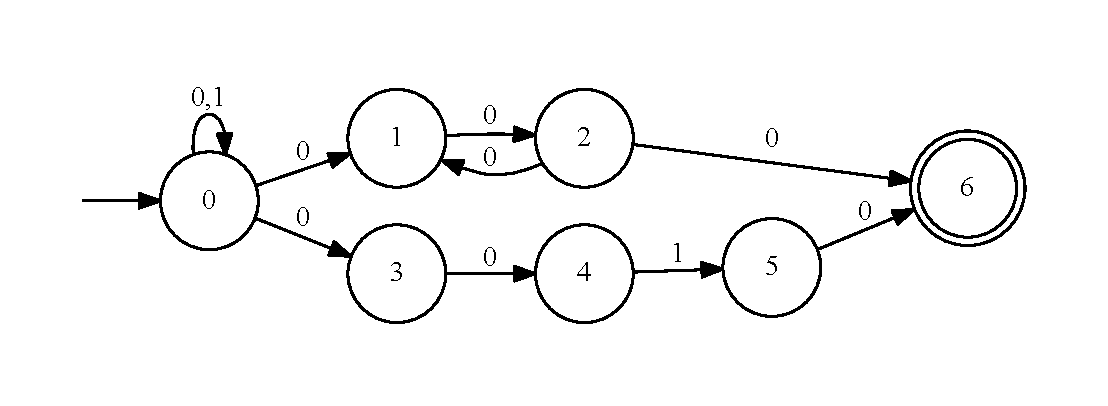
\includegraphics[width=\textwidth]{bilder/nfa_beispiel.pdf}
	\caption{Visuelle Darstellung des NFAs zum regulären Ausdruck \texttt{(0|1)*((00)+|001)0}}
	\label{nfa_beispiel}
\end{figure}

\begin{figure}[ht]
	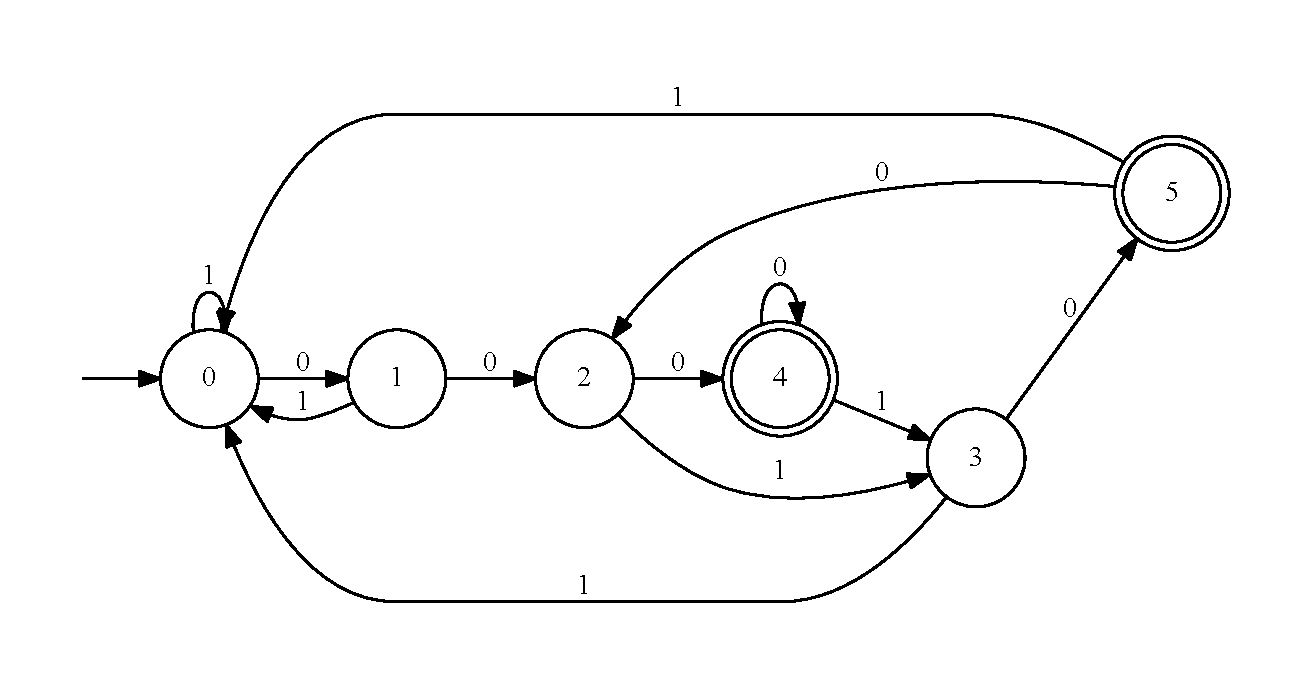
\includegraphics[width=\textwidth]{bilder/dfa_beispiel.pdf}
	\caption{Visuelle Darstellung des DFAs zum regulären Ausdruck \texttt{(0|1)*((00)+|001)0}}
	\label{dfa_beispiel}
\end{figure}

\section{Durchführung eines Musterabgleichs}

Der vorgestellte DFA lässt sich als zweidimensionale Übergangstabelle darstellen, die für einen gegebenen Ausgangszustand und ein gelesenes Eingabezeichen den Folgezustand zurückliefert.
Beginnend mit dem Startzustand muss somit lediglich für jedes Zeichen des Eingabewortes der aktuelle Zustand entsprechend der Tabelle angepasst werden und es kann am Ende überprüft werden, ob ein akzeptierender Zustand erreicht wurde.
Dieses Verfahren wird in Listing \ref{dfa_matching} schematisch dargestellt.

\begin{lstlisting}[language=Python,
caption=Durchführung des Musterabgleichs mithilfe eines DFA,
label=dfa_matching]
dfa = [[1, 0],
	[2, 0],
	[4, 3],
	[5, 0],
	[4, 3],
	[2, 0]]
cs = 0
accepting = [4, 5]

word = "010010"

for c in word:
	cs = dfa[cs][int(c)]

if cs in accepting:
	print("Word matches regular expression!")
\end{lstlisting}

\begin{lstlisting}[language=Python,
caption=Durchführung des Musterabgleichs mithilfe eines NFA,
label=nfa_matching]
nfa = [[[0, 1, 3], [0]],
	[[2], []],
	[[1, 6], []],
	[[4], []],
	[[], [5]],
	[[6], []],
	[[], []]]
cs = [0]
accepting = [6]

word = "010010"

for c in word:
	newCs = []
	for s in cs:
		newCs = newCs + nfa[s][int(c)]
	cs = newCs

for s in cs:
	if s in accepting:
		print("Word matches regular expression!")
		break
\end{lstlisting}

Listing \ref{nfa_matching} stellt entsprechend das Verfahren zur Durchführung des Musterabgleichs mittels eines NFAs dar.
Dieses funktioniert sehr ähnlich zu einem DFA, allerdings müssen gegebenenfalls mehrere Zustände gleichzeitig betrachtet werden, wodurch die Auswertung des Automaten komplizierter und zeitaufwändiger wird.

\section{Auswahl eines geeigneten Ansatzes}

Der Nachteil bei der Verwendung von NFAs liegt darin, dass teilweise mehrere Zustände gleichzeitig aktiv sind, da verschiedene Pfade auf einmal verfolgt werden müssen.
Dadurch steigt die Rechenlast beim Lesen von Zeichen und die allgemeine Performanz sinkt.
Bei DFAs ist dies nicht der Fall, da durch den Determinismus zu jeder Zeit klar ist, welche Transition verfolgt werden muss und in welchem Zustand der Automat sich befindet.

Der Nachteil eines DFA liegt allerdings darin, dass dieser im Gegensatz zum NFA eine exponentiell große Anzahl von Zuständen haben kann.
die Zeit für das Verarbeiten eines Strings wird dadurch zwar nicht direkt beeinflusst, allerdings steigt der Speicherverbrauch enorm, wodurch die Verwendung eines DFAs gegebenenfalls unmöglich wird.

Vergangene Arbeiten zeigen, dass ein unkomprimierter DFA die optimale Laufzeit erzielt \ref{Yu2013}.
Außerdem ist nicht zu erwarten, dass im Kontext einer Datenbankanfrage ein hoch komplexer regulärer Ausdruck benötigt wird, sodass der Automat eine effiziente Größe überschreiten würde.
Der exponentiellen Anzahl von Zuständen kann außerdem entgegen gewirkt werden, indem der Automat vor der Verwendung minimiert wird, was in den meisten Anwendungsfällen einen kompakten Automaten ergibt.

	\chapter{Paralleler Musterabgleich mit regulären Ausdrücken}
\label{sec:regex_naiv}

Aufbauend auf Kapitel \ref{sec:equals_naiv} wird im Folgenden eine komplexere Operation in Form eines Matchers für reguläre Ausdrücke im Kontext der in Kapitel \ref{sec:pipelining} beschriebenen kompilierten Anfragepipelines auf GPUs untersucht.
Diese Operation stellt ebenfalls eine Selektion über eine Spalte von String-Daten dar, bei der alle Tupel in die Ergebnisrelation übernommen werden, welche dem Muster eines vorgegebenen regulären Ausdrucks entsprechen.

Zunächst wird dazu erläutert, warum das Umsetzen einer solchen Operation im Kontext von Datenbanksystemen relevant ist.
Anschließend wird die allgemeine Struktur der Operation dargestellt, gefolgt von der tatsächlichen Umsetzung des Musterabgleichs mithilfe von Automaten.
Schließlich werden noch einige alternative Verfahren vorgestellt, welche unterschiedliche Eigenschaften aufweisen und mit der vorgestellten Umsetzung verglichen werden.

\section{Struktur der Operation}

Für das Verarbeiten des regulären Ausdrucks wird ein deterministischer Automat erstellt, der genau dann akzeptiert, wenn der aktuell überprüfte String in das Muster des regulären Ausdrucks passt.

Das allgemeine Vorgehen der Operation ist ähnlich zu dem in Kapitel \ref{sec:equals_umsetzung} beschriebenen einfachen String-Vergleich.
Jedem Thread der GPU wird ein Tupel zugewiesen, welches mithilfe des Automaten untersucht werden soll.
Nachdem der aktuelle Zustand des DFA auf den Startzustand gesetzt wurde, wird der String Zeichen für Zeichen durchlaufen, wobei der Zustand in jedem Schritt entsprechend der Regeln des Automaten aktualisiert wird.
Sobald die Zeichenkette vollständig durchlaufen wurde, wird geprüft, ob sich der Automat in einem akzeptierenden Zustand befindet, in welchem Fall der gesuchte String in das Muster des regulären Ausdrucks passt.
Ist am Ende kein akzeptierender Zustand erreicht, oder wurde die Untersuchung vorzeitig abgebrochen, weil ein Fehlerzustand erreicht wurde, wird das Tupel nicht in das Ergebnis übernommen.

Bei der Ausführung wird der gesamte Warp parallel abgearbeitet, wodurch die Positionen, an denen die Strings untersucht werden, für alle Lanes identisch sind.
Außerdem wird das Ergebnis erst geschrieben, sobald alle Threads ihren String vollständig durchlaufen haben oder einen Fehlerzustand erreicht haben.
Schließlich wird jedem Thread eine neue Zeichenkette zugewiesen, mit der das Verfahren wiederholt wird, bis sämtliche Tupel abgearbeitet sind.

\begin{figure}[]
	\begin{lstlisting}[language=MyC++]
	/* execute previous operators in the pipeline */
	
	char *p = data_content + char_offset[loop_var];
	char *pe = data_content + char_offset[loop_var + 1];
	
	int cs = machine_start;
	
	while(active) {
		cs = singleDfaStep(cs, p);
		
		p++;
		
		if (p == pe)		// string completely processed
			active = false;
		
		if (cs == 0)		// invalid state reached
			active = false;
	}
	
	active = cs >= machine_first_final;
	
	/* execute following operators in the pipeline */
	\end{lstlisting}
	\caption{Naive Implementierung einer Selektion mit einem regulären Ausdruck}
	\label{naive_regex}
\end{figure}

In Abbildung \ref{naive_regex} wird die Implementierung des Operators vorgestellt, der im Kontext der kompilierten Anfragepipelines die Selektion über einen regulären Ausdruck ausführt.
Die Datensätze \texttt{data\_content} und \texttt{char\_offset} enthalten wie in Kapitel \ref{sec:equals_umsetzung} die Zeichenketten aus der zu untersuchenden Spalte und die Indizes der einzelnen Tupel innerhalb des Datensatzes.

Zunächst wird die Lane initialisiert, indem ein Zeiger \texttt{p} auf den Anfang des zu untersuchenden Strings und der Zeiger \texttt{pe} auf das Ende gesetzt wird.
Außerdem wird der aktuelle Zustand \texttt{cs} auf den Startzustand des Automaten gesetzt.

In der Schleife wird anschließend über den gesamten String iteriert und dabei mithilfe der Methode \texttt{singleDfaStep} der Folgezustand des Automaten nach Einlesen des nächsten Zeichens bestimmt.
Daraufhin wird überprüft, ob der iterierende Zeiger \texttt{p} auf das Ende des Strings \texttt{pe} zeigt, in welchem Falle dieser vollständig durchlaufen wurde und die Lane vorerst deaktiviert werden kann.
Die Lane wird ebenfalls deaktiviert, wenn der Fehlerzustand \texttt{0} erreicht wurde, von dem aus ein Erreichen eines akzeptierenden Zustandes unmöglich ist.

Nachdem sämtliche Lanes ihre Berechnung abgeschlossen haben, wird überprüft, ob der aktuelle Zustand des DFA zu der Gruppe der akzeptierenden Zustände gehört.
Ist dies der Fall, wird die Lane für folgende Operationen aktiviert, ansonsten bleibt diese deaktiviert, sodass die Folgeoperationen nicht ausgeführt werden müssen.

\section{Erstellen und Durchlaufen des Automaten}
\label{sec:regex_duchlaufen}

Das vorgestellte Verfahren generiert vor der Ausführung des Anfrageplans einen deterministischen Automaten, welcher beim kompilieren der Anfragepipeline in den Kernel eingebaut wird.
Der Automat wird mithilfe des \emph{Ragel State Machine Compilers} \cite{Thurston2009} erzeugt, auf dem auch der Code zur Verarbeitung des Automaten basiert.

Ragel ermöglicht es, für das Auswerten eines gegebenen regulären Ausdrucks C-Code zu erzeugen, der automatisch in ein vorgegebenes Rahmenprogramm eingefügt wird.
Somit ist es leicht möglich, den Automaten in den Rahmen einer kompilierten Anfragepipeline einzupflegen, es müssen also keinerlei Schnittstellen zu anderen Sprachen oder Konzepten erstellt werden.

Der generierte Code lässt sich in zwei Hauptbestandteile aufteilen.
Zum einen wird etwas Code zur tatsächlichen Durchführung des Musterabgleichs generiert, welcher für unterschiedliche Ausdrücke größtenteils identisch ist.
Zum anderen werden einige Tabellen generiert, welche die tatsächlichen Zustände und Zustandsübergänge des Automaten beinhalten und für jeden regulären Ausdruck neu generiert werden.

\begin{figure}[]
	 \begin{lstlisting}[language=MyC++]
	 __device__ int singleDfaStep(int cs, char* p) {
		 int _slen;
		 int _trans;
		 const char *_keys;
		 const char *_inds;
		 
		 _keys = _machine_trans_keys + (cs<<1);
		 _inds = _machine_indicies + _machine_index_offsets[cs];
		 
		 _slen = _machine_key_spans[cs];
		 _trans = _inds[ _slen > 0 && _keys[0] <=(*p) &&
			 (*p) <= _keys[1] ?
			 (*p) - _keys[0] : _slen ];
		 
		 return _machine_trans_targs[_trans];
	 }
	 \end{lstlisting}
	 \caption{Methode zur Durchführung eines DFA-Schrittes}
	 \label{naive_regex_singledfastep}
\end{figure}
 
 Abbildung \ref{naive_regex_singledfastep} zeigt die Methode zur Durchführung eines DFA-Schrittes, welche in Abbildung \ref{naive_regex} verwendet wird.
 Die Implementierung basiert auf dem durch Ragel erzeugten Ausführungscode, welcher mit der \emph{flat}-Einstellung generiert wurde.
 Dies stellt den simpelsten Code dar, der von Ragel generiert wird, welcher sehr ähnlich zu dem in Kapitel \ref{sec:regex} vorgestellten Prinzip ist.
 Hier werden die ebenfalls von Ragel generierten und in Abbildung \ref{naive_regex_felder} dargestellten Felder verwendet, welche den eigentlichen DFA enthalten.
 In diesem Beispiel handelt es sich um den Automaten, der aus dem Ausdruck \texttt{(0|1)*((00)+|001)0} generiert wurde.
 
 \begin{figure}[]
	 \begin{lstlisting}[language=MyC++]
	static const char _machine_trans_keys[] = {
		0, 0, 0, 1, 0, 1, 0, 1, 0, 1, 0, 1, 0, 1, 0
	};
	
	static const char _machine_key_spans[] = {
		0, 2, 2, 2, 2, 2, 2
	};
	
	static const char _machine_index_offsets[] = {
		0, 0, 3, 6, 9, 12, 15
	};
	
	static const char _machine_indicies[] = {
		0, 2, 1, 3, 2, 1, 4, 
		5, 1, 6, 2, 1, 4, 5, 1, 
		3, 2, 1, 0
	};
	
	static const char _machine_trans_targs[] = {
		2, 0, 1, 3, 5, 4, 6
	};
	
	static const int machine_start = 1;
	static const int machine_first_final = 5;
	\end{lstlisting}
	\caption{Generierte Felder, die den DFA enthalten}
	\label{naive_regex_felder}
\end{figure}
 
Da diese Darstellung des Automaten für den Menschen kaum lesbar ist und ein Debugging somit sehr aufwändig wäre, bietet Ragel außerdem ein Werkzeug zur Visualisierung des Graphen.
Die vorher gezeigte Abbildung \ref{dfa_beispiel} zeigt dazu die visuelle Darstellung des erzeugten DFA.

\section{Alternative Verfahren}
\label{sec:regex_alternativen}

Zusätzlich zur \emph{flat}-Einstellung bietet Ragel die \emph{Table}-Option, welche eine Generierung von Code erlaubt, welche für die Verarbeitung regulärer Ausdrücke mit einem großen Alphabet optimiert wurde.
Im Gegensatz zur \emph{flat}-Einstellung wird nicht das aktuell untersuchte Zeichen als Index für einen Array von Zustandsübergängen verwendet, sondern in einem Feld eine binäre Suche nach der korrekten Transition durchgeführt.
Nach Thurston ist die oben beschriebene \emph{flat}-Option generell schneller, sie lässt sich allerdings nur für ein kleines Alphabet anwenden \cite{Thurston2009}.
Da im Datenbankkontext generell eher simplere Ausdrücke zu erwarten sind, ist es für die meisten Anwendungsfälle zwar ausreichend, die einfache und schnelle Implementierung zu wählen.
Es ist aber auch interessant zu untersuchen, wie groß der Leistungsverlust mit der alternativen Implementierung aussieht, falls komplexere Ausdrücke untersucht werden sollen.

Als Alternative zur vollumfänglichen Unterstützung von regulären Ausdrücken bieten viele Datenbankmanagementsysteme den \emph{LIKE}-Operator an, welcher den einfachen String-Vergleich um Platzhalter erweitert.
So ist es dem Nutzer möglich, anstelle des genauen Suchstrings ein Muster anzugeben, in dem Platzhalter für beliebige Zeichen enthalten sind.
Mithilfe dieser simpel umzusetzenden Operation lassen sich viele einfache Abfragen an eine Datenbank modellieren, sodass in vielen Fällen kein richtiger regulärer Ausdruck benötigt wird.
Es ist daher interessant zu sehen, wie sich die Leistungsfähigkeit dieser Operation mit geringerem Funktionsumfang gegenüber der Umsetzung eines vollständigen Matchers für reguläre Ausdrücke verhält.
	\chapter{Verbesserung des Verfahrens zum Musterabgleich}

Bei dem in Kapitel \ref{sec:regex_naiv} vorgestellten Verfahren tritt ein ähnliches Problem auf wie bei dem zuvor beschriebenen, einfachen String-Vergleich.
Aufgrund der unterschiedlichen Struktur von Strings werden einige Lanes innerhalb eines Warps früher als andere Lanes inaktiv wenn sie einen Fehlerzustand oder das Ende des Eingabestrings erreicht haben.
Dies hat eine Unterauslastung des Warps zur Folge, wodurch Rechenleistung verschwendet wird.
Aus diesem Grund ist es wünschenswert den inaktiv gewordenen Threads dynamisch neue Arbeit zuzuweisen.
Dazu wird das in Kapitel \ref{sec:equals_lane_refill} vorgestellte Lane Refill-Verfahren zum Einsatz kommen, wodurch im Rahmen der kompilierten Anfragepipelines die Laufzeit optimiert werden kann.


\section{Struktur des optimierten Musterabgleichs mit Lane Refill}

Die grundlegende Funktionsweise des Lane Refill wurde in Kapitel \ref{sec:equals_lane_refill_funktionsweise} beschrieben und ist genau so auch auf den parallelen Musterabgleich anwendbar.
Bei dem Musterabgleich wird eine Lane immer dann inaktiv, wenn der untersuchte String vollständig durchlaufen wurde oder ein Fehlerzustand erreicht wurde und es nicht mehr möglich ist, einen akzeptierenden Zustand zu erreichen.
Nach genau diesen Ereignissen muss überprüft werden, ob die gewünschte Auslastung des Warps unterschritten wird und gegebenenfalls die aktuellen Elemente in den Puffer geschrieben oder neue Elemente aus dem Puffer geladen werden.

Die allgemeine Struktur des Kernels ist identisch zu der in Abbildung \ref{equals_lane_refill_code} vorgestellten Struktur des einfachen String-Vergleichs.
Um den parallelen Musterabgleich damit umzusetzen, muss die innere Schleife so angepasst werden, dass statt einem einfachen Vergleich zweier Zeichen, der Zustand des Automaten angepasst wird.
Der gesamte Kernel ist in Anhang \ref{apx:regex_lane_refill} dargestellt.

Zunächst wird hier von allen aktiven Lanes ein Schritt im DFA durchgeführt und überprüft, ob ein Fehlerzustand erreicht wurde.
Anschließend wird für die vollständig durchlaufenen Strings überprüft, ob diese sich in einem akzeptierenden Zustand befinden und gegebenenfalls die Folgeoperationen der Pipeline ausgeführt.

Die technische Umsetzung der Puffer-Operationen funktioniert identisch zu dem in Kapitel \ref{sec:equals_lane_refill_pufferung} beschriebenen Vorgehen, mit dem Unterschied, dass hier der Inhalt der Variablen \texttt{p}, \texttt{pe} und \texttt{cs} im Puffer gespeichert werden.
Eine Reduzierung des Overheads durch die Puffer-Operation ist ebenfalls analog zu dem in Kapitel \ref{sec:unroll} vorgestellten Verfahren möglich.
	\chapter{Optimierung der Ausführungsparameter}

Die Ausführungszeit der in den vorherigen Kapiteln vorgestellten Algorithmen wird stark durch unterschiedliche Parameter beeinflusst.
Den größten Einfluss nimmt dabei die Art des Datensatzes, also wie viele Matches er enthält, wie lang die enthaltenen Zeichenketten sind, wie viele Strings im Datensatz vorhanden sind und wie die Matches darin verteilt sind.
Wie sehr unterschiedliche Datensätze die Ausführungszeit beeinflussen, soll in Kapitel \ref{sec:equals_evaluation} untersucht werden.

Neben den Eigenschaften des Datensatzes gibt es noch Parameter, die bei der Ausführung des Algorithmus der GPU übermittelt werden und dort ebenfalls einen erheblichen Einfluss auf die Laufzeit nehmen.
Diese Parameter bestehen, wie in Kapitel \ref{sec:cuda_scheduling} beschrieben, in der Anzahl der Threads pro Block (\emph{Block Size}) und der Anzahl der Blöcke im Grid (\emph{Grid Size}).
Aus den Parametern setzt sich die \emph{Grid-Konfiguration} zusammen, die durch das Ausprobieren unterschiedlicher Werte praktisch optimiert werden kann.

\begin{figure}[ht]
	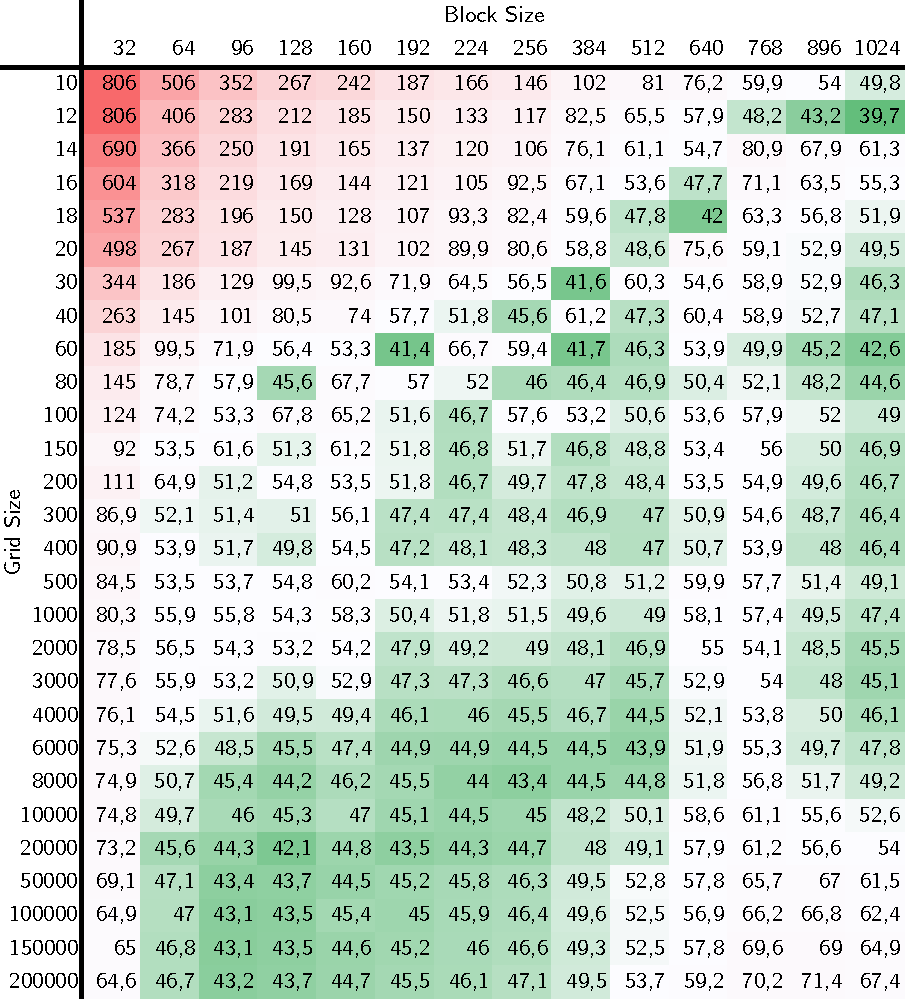
\includegraphics[]{bilder/parameter025.pdf}
	\caption{Laufzeit des naiven String-Vergleichsalgorithmus in Millisekunden für den Type-Datensatz mit einer Selektivität von 0.25\% unter Verwendung unterschiedlicher Grid-Konfigurationen}
	\label{parameter025}
\end{figure}

Um dieses Vorgehen zu veranschaulichen, soll anhand eines Beispiels gezeigt werden, wie eine möglichst gute Grid-Konfiguration gefunden werden kann und welchen Einfluss unterschiedliche Konfigurationen auf die Laufzeit haben.
Abbildung \ref{parameter025} zeigt dazu die Laufzeit für den String-Vergleichsalgorithmus in Millisekunden, welcher für unterschiedliche Grid-Konfigurationen auf dem in Kapitel \ref{sec:equals_evaluation_workloads} vorgestellten Type-Datensatz mit einer Selektivität von 0.25\% ausgeführt wurde.
Besonders hohe Laufzeiten sind dabei rot und besonders geringe Laufzeiten grün eingefärbt.

Es fällt auf, dass eine niedrige Block Size in Kombination mit einer niedrigen Grid Size zu einer hohen Laufzeit führt.
Außerdem gibt es bei einer Grid Size von unter 100 einige Kombinationen, die besonders geringe Laufzeiten aufweisen, allerdings von weniger guten Konfigurationen umgeben sind.
Mit einer Grid Size zwischen 2.000 und 200.000 in Verbindung mit einer Block Size zwischen 64 und 512 werden generell gute Laufzeiten erzielt.
Wird allerdings eine Block Size über 512 gewählt, nimmt die Leistungsfähigkeit des Systems wieder ab.

Generell ist die Analyse eines solchen Ergebnisses schwierig, da die Grid-Konfiguration Einfluss auf unterschiedlichste Bereiche der GPU nimmt und der CUDA-Optimierer einige Effekte erfolgreich versteckt.
Die hohe Laufzeit des Algorithmus bei einer geringen Anzahl von Threads ist dadurch zu erklären, dass zunächst nicht alle Kerne der GPU ausgelastet sind, weil nicht genügend Warps für die Anzahl der Streaming Multiprocessors vorhanden sind.
Eine steigende Anzahl von Threads führt zwar dazu, dass alle Kerne ausgelastet sind, allerdings können bei Speicherzugriffen nicht genügend Warps vom Scheduler ausgetauscht werden, als dass die Latenz der Speicherzugriffe, wie in Kapitel \ref{sec:cuda_scheduling} beschrieben, erfolgreich versteckt werden könnte.
In dem zuvor beschriebenen Bereich, in dem ordentliche Laufzeiten erzielt werden, steht eine ausreichende Anzahl von Threads zur Verfügung, um eventuelle Latenzen zu verstecken und somit die GPU bestmöglich auszulasten.
Wie der Anstieg der Laufzeiten bei einer Block Size von über 512 zu begründen ist, ist an dieser Stelle unklar.

Für die Verwendung des Algorithmus sollte im Allgemeinen eine Grid-Konfiguration aus dem Bereich gewählt werden, der eine durchweg ordentliche Performanz erzielt.
Dadurch wird mit hoher Wahrscheinlichkeit eine Konfiguration gewählt, mit der eine Laufzeit erreicht wird, die bis auf eine kleinere Abweichung dem Optimum entspricht.
Die Position des Bereichs ändert sich für unterschiedliche Selektivitäten des Datensatzes nur geringfügig, wie in zahlreichen Tests untersucht wurde und beispielhaft in Anhang \ref{apx:parameter64} für eine Selektivität von 64\% analog zu Abbildung \ref{parameter025} dargestellt wird.
Aus diesem Grund kann die Grid-Konfiguration schon vor der Ausführung bestimmt werden und eine nah am Maximum liegende Leistungsfähigkeit erzielt werden.
Bei den Leistungsmessungen in den folgenden Kapiteln sollte sich allerdings nicht darauf verlassen werden, dass durch diese Annäherung ein nahezu optimaler Wert gefunden wird, weshalb für die Tests jeweils das Optimum aus einer Auswahl von Grid-Konfigurationen bestimmt wird.
Dazu werden alle Konfigurationen mit einer Grid Size von $G=\{1.000, 2.000, 3.000, 4.000, 6.000, 8.000, 10.000, 20.000, 50.000,$ $100.000, 150.000, 200.000\}$ und einer Block Size von $B=\{32, 64, 96, 128, 160, 192, 224, 256,$ $384, 512, 640, 768\}$ überprüft und das Optimum der Messungen für die Auswertung der folgenden Experimente gewählt.
	\chapter{Evaluation des einfachen String-Vergleichs}

In Kapitel \ref{sec:equals_lane_refill} wurde eine Technik vorgestellt, von der zu erwarten ist, dass sie die Laufzeit des einfachen String-Vergleichs verbessert, indem die Ressourcen der GPU besser genutzt werden und somit eine erhöhte Auslastung erreicht wird.
Da diese Technik allerdings einen gewissen Overhead mit sich bringt, bleibt es noch zu untersuchen, ob diese Technik tatsächlich eine bessere Laufzeit erzielt, oder ob der Mehraufwand so groß ist, dass die erreichten Vorteile von diesem überschattet werden.
In diesem Kapitel wird diese Untersuchung anhand realer Arbeitslasten durchgeführt und außerdem überprüft, ob die in Kapitel \ref{sec:unroll} vorgestellte Reduzierung des Overheads eine weitere Leistungssteigerung mit sich bringt.

\section{Testumgebung}

Für die Durchführung der Leistungsmessungen wird der Algorithmus so angepasst, dass dieser lediglich die Anzahl der passenden Zeichenketten zählt und diese am Ende ausgibt.
Die Testumgebung entspricht also einer Selektion auf einer Spalte einer Relation und dem anschließenden Zählen der Ergebnisse.
Dieses Vorgehen hat den Vorteil, dass das Zählen der Ergebnisse nicht viel Rechenaufwand verursacht und somit das Ergebnis möglichst wenig verfälscht wird.
Trotzdem bleibt es aber möglich aufgrund der Ausgabe des Algorithmus beurteilen zu können, ob der Test korrekt durchgeführt wurde.

Sämtliche Tests wurden auf einem Computer durchgeführt, welcher eien NVIDIA GTX 950 verbaut hat und als Betriebssystem Ubuntu 18.04 verwendet.

\section{Verwendete Workloads und deren Merkmale}

In analytischen Anwendungsfällen kommen häufig selektive Filter vor \cite{Boncz2013}, weshalb diese ebenfalls für diese Untersuchungen verwendet werden.
Außerdem ist zu erwarten, dass diese besonders stark vom Lane-Refill profitieren werden, da bei einer kleinen Menge von Ergebnissen oftmals eine starke Unterauslastung auftritt.

Der erste verwendete Workload, welcher im Folgenden \emph{Type} genannt wird, wurde aus dem TPC-H-Benchmark entnommen.\footnote{\url{http://www.tpc.org/tpch/}}.
Hier wird eine Selektion über die Type-Spalte durchgeführt, welche Zeichenketten der Länge 16-25 enthält.
Diese bestehen aus den Zeichen \emph{A-Z} und dem Leerzeichen.
Für die Untersuchung wurde ein Datensatz mit 90.000.000 Tupeln generiert.

Ein weiterer Workload wurde aus dem Datensatz von DBLP erstellt, welcher die Titel vieler Veröffentlichungen im Informatik-Umfeld enthält.
Dazu wurden doppelte Titel entfernt und die übrigen Strings so angepasst, dass diese nur noch Kleinbuchstaben enthalten.
Die durchschnittliche Länge der Zeichenketten in diesem Datensatz beträgt 76 Zeichen und es wurde ein Präfix untersucht, welcher 31 Zeichen beinhaltet.
Der generierte Datensatz enthält schließlich 21.513.695 Tupel.

Um die unterschiedlichen Selektivitäten für die folgenden Tests zu erreichen wurde ein neuer String entsprechend zufällig verteilt in den Datensatz eingebracht.
Die gewünschte Datengröße wurde schließlich erreicht, indem der so generierte Datensatz einige male vervielfacht wurde.

\section{Vorstellung der Messergebnisse}

\begin{figure}[ht]
	\centering
	\begin{tikzpicture}
		\begin{axis}[
			ybar,		% Säulendiagramm
			xlabel={Anteil Matches},	% Achsenbeschriftung
			xtick=data,
			xticklabels from table={daten/type_equals.csv}{Selectivity},	% Beschriftung der Markierungen 
			width=\textwidth,	% Diagrammbreite
			bar width=0.2cm,	% Breite der Säulen
			ylabel={Laufzeit (ms)},	% Achsenbeschritung
			ymin=0,		% Säulen stehen auf der X-Achse
			%legend style={at={(0,0)}}
			legend pos=north west,		% Legende am oberen linken Rand positionieren
			legend style={legend cell align=left} % Text linksbündig anordnen
			]
			\addplot table [x expr=\coordindex, y=equals]{daten/type_equals.csv}; 
			\addlegendentry{Naiv};
			\addplot table [x expr=\coordindex, y=buffer]{daten/type_equals.csv};
			\addlegendentry{Mit Lane Refill}
			\addplot table [x expr=\coordindex, y=unroll_2]{daten/type_equals.csv};
			\addlegendentry{In Zweierschritten}
			\addplot table [x expr=\coordindex, y=unroll_3]{daten/type_equals.csv};
			\addlegendentry{In Dreierschritten}
		\end{axis}
	\end{tikzpicture}
	\caption{Laufzeit für Gleichheitstest mit verschiedener Verteilung beim Type-Benchmark}
	\label{fig:type_equals}
\end{figure}

\begin{figure}[ht]
	\centering
	\begin{tikzpicture}
		\begin{axis}[
			ybar,		% Säulendiagramm
			xlabel={Anteil Matches},	% Achsenbeschriftung
			xtick=data,
			xticklabels from table={daten/type_prefix.csv}{Selectivity},	% Beschriftung der Markierungen 
			width=\textwidth,	% Diagrammbreite
			bar width=0.4cm,	% Breite der Säulen
			ylabel={Laufzeit (ms)},	% Achsenbeschritung
			ymin=0,		% Säulen stehen auf der X-Achse
			legend pos=north west,		% Legende am oberen linken Rand positionieren
			legend style={legend cell align=left} % Text linksbündig anordnen
			]
			\addplot table [x expr=\coordindex, y=equals]{daten/type_prefix.csv}; 
			\addlegendentry{Naiv};
			\addplot table [x expr=\coordindex, y=buffer]{daten/type_prefix.csv};
			\addlegendentry{Mit Lane Refill}
		\end{axis}
	\end{tikzpicture}
	\caption{Laufzeit für Präfixtest mit verschiedener Verteilung beim Type-Benchmark}
\label{fig:type_prefix}
\end{figure}

\begin{figure}[ht]
	\centering
	\begin{tikzpicture}
		\begin{axis}[
			ybar,		% Säulendiagramm
			xlabel={Anteil Matches},	% Achsenbeschriftung
			xtick=data,
			xticklabels from table={daten/dblp_prefix.csv}{Selectivity},	% Beschriftung der Markierungen 
			width=\textwidth,	% Diagrammbreite
			bar width=0.4cm,	% Breite der Säulen
			ylabel={Laufzeit (ms)},	% Achsenbeschritung
			ymin=0,		% Säulen stehen auf der X-Achse
			legend pos=north west,		% Legende am oberen linken Rand positionieren
			legend style={legend cell align=left} % Text linksbündig anordnen
			]
			\addplot table [x expr=\coordindex, y=equals]{daten/dblp_prefix.csv}; 
			\addlegendentry{Naiv};
			\addplot table [x expr=\coordindex, y=buffer]{daten/dblp_prefix.csv};
			\addlegendentry{Mit Lane Refill}
		\end{axis}
	\end{tikzpicture}
	\caption{Laufzeit für Präfixtest mit verschiedener Verteilung beim DBLP-Benchmark}
\label{fig:dblp_prefix}
\end{figure}

\section{Diskussion der Ergebnisse}

	\chapter{Evaluation des parallelen Musterabgleichs}

Nachdem im letzten Kapitel gezeigt wurde, dass das Lane Refill-Verfahren eine erhöhte Leistungsfähigkeit des einfachen String-Vergleichs erreicht, bleibt nun zu untersuchen, wie sich die vorgestellten Methoden zum parallelen Musterabgleich damit verhalten.
Zunächst soll geklärt werden, welcher der vorgestellten Algorithmen ohne tiefgreifende Verbesserungen die beste Laufzeit erzielen kann.
Im Anschluss wird untersucht, welcher Algorithmus am meisten vom Lane Refill profitiert und ob sich die Beobachtungen für unterschiedlich geartete reguläre Ausdrücke ändert.
Die Testumgebung ist dabei identisch zu dem im Kapitel \ref{sec:equals_testumgebung} beschriebenen Aufbau.

\section{Verwendete Workloads und deren Merkmale}

Für die ersten Tests wurde der in \ref{sec:equals_evaluation_workloads} vorgestellte DBLP-Datensatz verwendet.
Dieser eignet sich optimal zur Untersuchung der Laufzeitverbesserung durch das Lane Refill, da dieser analytische Workload mit variabler Selektivität Analysen zu verschiedenen Stufen der Unterauslastung ermöglicht.
Außerdem bietet sich dieser Datensatz an, da ein Vergleich zwischen dem einfachen Präfixtest und dem Präfixtest mittels regulärer Ausdrücke durchgeführt werden kann.

Ein weiterer Workload wurde dem TPC-H-Benchmark entnommen, in dem eine Selektion über die \emph{Name}-Spalte der \emph{Products}-Relation durchgeführt wird.
Die enthaltenen Strings haben eine Länge zwischen 26 und 43 Zeichen, welche aus den Kleinbuchstaben \emph{a-z} und dem Leerzeichen bestehen.
Der Datensatz wurde einige male repliziert, sodass dieser 46.000.000 Tupel enthält.

\section{Vorstellung der Messergebnisse}

Abbildungen \ref{fig:regex_dblpANY_no_buffer} bis \ref{fig:regex_p_name} zeigen die Laufzeiten der verschiedenen Algorithmen in den entwickelten Benchmarks.
Für ein einfacheres Verständnis werden besondere Auffälligkeiten dazu aufgezeigt und im nächsten Abschnitt analysiert.

\subsection{Vergleich der Basisalgorithmen mit dem DBLP-Datensatz}
\label{sec:regex_evaluation_beobachtung_1}

Bei der ersten Messung soll überprüft werden, wie sich die in Kapitel \ref{sec:regex_naiv} vorgestellten Verfahren zur Durchführung eines einfachen Musterabgleichs ohne tiefgreifende Verbesserungen wie dem Lane Refill-Verfahren verhalten.
Untersucht werden hier die in Kapitel \ref{sec:regex_duchlaufen} beschriebene \emph{Flat}-Variante des von Ragel generierten Algorithmus, die in Kapitel \ref{sec:regex_alternativen} vorgestellte \emph{Table}-Variante dieses Verfahrens, die dort ebenfalls angesprochene \emph{LIKE}-Operation, welche aus DogQC entnommen wurde und die in Kapitel \ref{sec:prefixtest} vorgestellte Implementierung zum einfachen Präfixtest.
Der untersuchte reguläre Ausdruck passt auf eine bestimmte Zeichenfolge am Anfang jedes Strings und lässt keine Zeichen vor diesem Suchstring zu, danach sind dagegen beliebige Strings zulässig. 

\begin{figure}[ht]
	\centering
	\begin{tikzpicture}
		\begin{axis}[
			ybar,		% Säulendiagramm
			xlabel={Anteil Matches},	% Achsenbeschriftung
			xtick=data,
			xticklabels from table={daten/regex_dblpANY_no_buffer.csv}{Selectivity},	% Beschriftung der Markierungen 
			width=\textwidth,	% Diagrammbreite
			height=300, % Diagrammhöhe
			bar width=0.2cm,	% Breite der Säulen
			ylabel={Laufzeit (ms)},	% Achsenbeschritung
			ymin=0,		% Säulen stehen auf der X-Achse
			%legend style={at={(0,0)}}
			legend pos=north west,		% Legende am oberen linken Rand positionieren
			legend style={legend cell align=left} % Text linksbündig anordnen
			]
			\addplot table [x expr=\coordindex, y=flat]{daten/regex_dblpANY_no_buffer.csv}; 
			\addlegendentry{Flat};
			\addplot table [x expr=\coordindex, y=table]{daten/regex_dblpANY_no_buffer.csv};
			\addlegendentry{Table}
			\addplot table [x expr=\coordindex, y=equals]{daten/regex_dblpANY_no_buffer.csv};
			\addlegendentry{Präfix}
			\addplot table [x expr=\coordindex, y=like]{daten/regex_dblpANY_no_buffer.csv};
			\addlegendentry{Like}
		\end{axis}
	\end{tikzpicture}
	\caption{Laufzeit für Präfixtest mit Basisalgorithmen für den DBLP-Datensatz}
	\label{fig:regex_dblpANY_no_buffer}
\end{figure}

Bei den in Abbildung \ref{fig:regex_dblpANY_no_buffer} dargestellten Ergebnissen fällt zunächst auf, dass die Ausführungszeit aller Algorithmen für einen größeren Anteil Matches monoton ansteigt.
Die beiden Implementierungen, welche reguläre Ausdrücke verwenden, werden ab einem Anteil von 8\% kaum noch langsamer, wogegen die Geschwindigkeit der anderen beiden Verfahren dabei immer schneller sinkt.
Die \emph{Flat}-Variante ist zwischen 15\% und 22\% schneller als die \emph{Table}-Variante der Ragel-Umsetzung, wobei der Unterschied für mittelgroße Selektivitäten am größten ist.
Der \emph{LIKE}-Operator aus DogQC ist zwischen 1\% und 13\% schneller als der Präfixtest, wobei der Unterschied für einen höheren Anteil Matches größer wird.
Der Präfixtest ist bei einer Selektivität von unter 32\% zwischen 50\% und 65\% schneller als die \emph{Flat}-Variante.
Bei einem Anteil Matches von 64\% beträgt dieser Unterschied 37\%.

\subsection{Verbesserung der Algorithmen durch das Lane Refill}
\label{sec:regex_evaluation_beobachtung_2}

Die nachfolgende Untersuchung dient dazu, den Einfluss des Lane Refill auf die Varianten \emph{Flat} und \emph{Table} des regulären Musterabgleichs sowie den einfachen Präfixtest zu analysieren.
Der hier verwendete reguläre Ausdruck ist derselbe wie im vorherigen Abschnitt.

\begin{figure}[ht]
	\centering
	\begin{tikzpicture}
		\begin{axis}[
			ybar,		% Säulendiagramm
			xlabel={Anteil Matches},	% Achsenbeschriftung
			xtick=data,
			xticklabels from table={daten/regex_dblpANY_buffer.csv}{Selectivity},	% Beschriftung der Markierungen 
			width=\textwidth,	% Diagrammbreite
			height=300, % Diagrammhöhe
			bar width=0.2cm,	% Breite der Säulen
			ylabel={Verbesserung durch Lane Refill (\%)},	% Achsenbeschritung
			ymin=0,		% Säulen stehen auf der X-Achse
			%legend style={at={(0,0)}}
			legend pos=north west,		% Legende am oberen linken Rand positionieren
			legend style={legend cell align=left} % Text linksbündig anordnen
			]
			\addplot table [x expr=\coordindex, y=flat]{daten/regex_dblpANY_buffer.csv}; 
			\addlegendentry{Flat};
			\addplot table [x expr=\coordindex, y=table]{daten/regex_dblpANY_buffer.csv};
			\addlegendentry{Table}
			\addplot table [x expr=\coordindex, y=equals]{daten/regex_dblpANY_buffer.csv};
			\addlegendentry{Präfix}
		\end{axis}
	\end{tikzpicture}
	\caption{Verbesserungen der Algorithmen durch das Lane Refill für den DBLP-Datensatz}
	\label{fig:regex_dblpANY_buffer}
\end{figure}

Abbildung \ref{fig:regex_dblpANY_buffer} zeigt dazu die Verbesserung der Laufzeit, welche durch das Einbinden des Lane Refill-Verfahrens in die Basisalgorithmen erreicht wird.
Bei den beiden Verfahren, die auf dem regulären Musterabgleich basieren, ist eine bedeutend größere Verbesserung zu sehen, als bei dem Präfixtest.
Beide auf Ragel basierenden Algorithmen werden in ähnlichem Maße durch das Lane Refill verbessert, wobei die \emph{Flat}-Variante etwas mehr davon profitiert.
Bis zu einer Selektivität von 16\% beträgt die Verbesserung der beiden Verfahren für den Musterabgleich mehr als 50\% gegenüber der ursprünglichen Laufzeit.
Die Verbesserung aller untersuchter Algorithmen ist für einen mittelgroßen Anteil Matches am größten und fällt besonders für größere Anteile stark ab.

\subsection{Vergleich der optimierten Algorithmen}
\label{sec:regex_evaluation_beobachtung_3}

Schließlich werden die absoluten Laufzeiten der durch das Lane Refill verbesserten Verfahren untereinander und mit dem \emph{LIKE}-Operator verglichen.
Der reguläre Ausdruck bleibt derselbe wie in den letzten beiden Abschnitten beschrieben.

\begin{figure}[ht]
	\centering
	\begin{tikzpicture}
		\begin{axis}[
			ybar,		% Säulendiagramm
			xlabel={Anteil Matches},	% Achsenbeschriftung
			xtick=data,
			xticklabels from table={daten/regex_dblpANY_optimal.csv}{Selectivity},	% Beschriftung der Markierungen 
			width=\textwidth,	% Diagrammbreite
			height=300, % Diagrammhöhe
			bar width=0.2cm,	% Breite der Säulen
			ylabel={Laufzeit (ms)},	% Achsenbeschritung
			ymin=0,		% Säulen stehen auf der X-Achse
			%legend style={at={(0,0)}}
			legend pos=north west,		% Legende am oberen linken Rand positionieren
			legend style={legend cell align=left} % Text linksbündig anordnen
			]
			\addplot table [x expr=\coordindex, y=flat-buffer]{daten/regex_dblpANY_optimal.csv}; 
			\addlegendentry{Flat mit Lane Refill};
			\addplot table [x expr=\coordindex, y=table-buffer]{daten/regex_dblpANY_optimal.csv};
			\addlegendentry{Table mit Lane Refill}
			\addplot table [x expr=\coordindex, y=equals-buffer]{daten/regex_dblpANY_optimal.csv};
			\addlegendentry{Präfix mit Lane Refill}
			\addplot table [x expr=\coordindex, y=like]{daten/regex_dblpANY_optimal.csv};
			\addlegendentry{Like}
		\end{axis}
	\end{tikzpicture}
	\caption{Laufzeiten der optimierten Algorithmen für den DBLP-Datensatz}
	\label{fig:regex_dblpANY_optimal}
\end{figure}

Die in Abbildung \ref{fig:regex_dblpANY_optimal} dargestellten Laufzeiten aller Algorithmen steigen für einen höheren Anteil von Matches monoton an.
Im Allgemeinen liefert der durch das Lane Refill verbesserte Präfixtest die beste Laufzeit, was nur nicht für eine Selektivität von 64\% gilt.
Für eine steigende Anzahl passender Matches steigen die gepufferten Operationen besonders stark an, weshalb die ungepufferte \emph{LIKE}-Implementierung für hohe Selektivitäten eine vergleichsweise geringe Laufzeit bietet, obwohl diese für niedrige Selektivitäten zu den langsamsten gehört.
Die \emph{Flat}-Variante des regulären Musterabgleichs bietet stets eine geringere Laufzeit als die entsprechende \emph{Table}-Variante.

\subsection{Einfluss beliebiger Anfangszeichen in dem DBLP-Datensatz}
\label{sec:regex_evaluation_beobachtung_4}

Als nächstes wird untersucht, wie sich die Laufzeiten der Algorithmen entwickeln, wenn beliebige Zeichen vor dem gesuchten String stehen dürfen.
Der Datensatz bleibt dazu identisch zu den vorherigen Tests, es wird lediglich der reguläre Ausdruck dementsprechend erweitert, dass dieser beliebige Zeichen vor dem Suchstring zulässt.
Diese Modifikation führt dazu, dass der Präfixtest an dieser Stelle nicht mehr untersucht werden kann, da dieser keine beliebigen Zeichen unterstützt.

\begin{figure}[ht]
	\centering
	\begin{tikzpicture}
		\begin{axis}[
			ybar,		% Säulendiagramm
			xlabel={Anteil Matches},	% Achsenbeschriftung
			xtick=data,
			xticklabels from table={daten/regex_ANYdblpANY.csv}{Selectivity},	% Beschriftung der Markierungen 
			width=\textwidth,	% Diagrammbreite
			height=300, % Diagrammhöhe
			bar width=0.15cm,	% Breite der Säulen
			ylabel={Laufzeit (ms)},	% Achsenbeschritung
			ymax=800,
			ymin=0,		% Säulen stehen auf der X-Achse
			%legend style={at={(0,0)}}
			legend pos=north east,		% Legende am oberen linken Rand positionieren
			legend style={legend cell align=left} % Text linksbündig anordnen
			]
			\addplot table [x expr=\coordindex, y=flat]{daten/regex_ANYdblpANY.csv}; 
			\addlegendentry{Flat};
			\addplot table [x expr=\coordindex, y=flat-buffer]{daten/regex_ANYdblpANY.csv};
			\addlegendentry{Flat mit Lane Refill}
			\addplot table [x expr=\coordindex, y=table]{daten/regex_ANYdblpANY.csv};
			\addlegendentry{Table}
			\addplot table [x expr=\coordindex, y=table-buffer]{daten/regex_ANYdblpANY.csv};
			\addlegendentry{Table mit Lane Refill}
			\addplot table [x expr=\coordindex, y=like]{daten/regex_ANYdblpANY.csv};
			\addlegendentry{Like}
		\end{axis}
	\end{tikzpicture}
	\caption{Laufzeiten für Benchmark, der beliebige Anfangszeichen zulässt}
	\label{fig:regex_ANYdblpANY}
\end{figure}

In Abbildung \ref{fig:regex_ANYdblpANY} ist zu erkennen, dass die Ausführungszeiten aller Algorithmen bis zu einer Selektivität von ungefähr 8\% unabhängig von der Anzahl der Matches im Ergebins sind.
Je höher die Selektivität wird, desto geringer wird die Ausführungszeit.
Beide Algorithmen, welche die \emph{Flat}-Einstellung von Ragel verwenden sind im Allgemeinen schneller als die entsprechenden Gegenstücke mit der \emph{Table}-Einstellung.
Am schnellsten ist hier die \emph{LIKE}-Operation aus DogQC.
Die Verbesserung der \emph{Flat}-Variante des Musterabgleichs durch das Lane Refill beträgt zwischen 26\% und 35\% und wird für eine höhere Anzahl von Matches größer.
Für die \emph{Table}-Variante beträgt die Verbesserung zwischen 17\% und 33\% und wird ebenfalls für höhere Anzahlen von Matches größer.

\subsection{Vergleich verschiedener Automatengrößen mit dem TPC-H-Datensatz}
\label{sec:regex_evaluation_beobachtung_5}

Zum Schluss wird untersucht, welchen Einfluss die Größe des Automaten auf die beiden Algorithmen zum parallelen Musterabgleich hat.
Dazu wurde eine Selektion über die \emph{Name}-Spalte der \emph{Products}-Relation aus dem TPC-H-Datensatz durchgeführt, wobei die Größe des Automaten variiert wurde.
Zu diesem Zweck wurde ein regulärer Ausdruck erstellt, welcher ein Suchwort annimmt und beliebige Zeichen vor und nach diesem Wort zulässt
Die Selektivität dieses Ausdrucks beträgt etwa 11\%.
Um die Automatengröße zu erhöhen, wurden weitere Suchwörter, welche in dieser Form nicht im Datensatz enthalten sind, mit dem bestehenden Ausdruck \emph{oder}-verknüpft.
Dadurch wird ein größerer Automat bei gleichbleibender Selektivität erreicht.


\begin{figure}[ht]
	\centering
	\begin{tikzpicture}
		\begin{axis}[
			ybar,		% Säulendiagramm
			xlabel={Anzahl Zustände},	% Achsenbeschriftung
			xtick=data,
			xticklabels from table={daten/regex_p_name.csv}{states},	% Beschriftung der Markierungen 
			width=\textwidth,	% Diagrammbreite
			height=300, % Diagrammhöhe
			bar width=0.4cm,	% Breite der Säulen
			ylabel={Laufzeit (ms)},	% Achsenbeschritung
			ymin=0,		% Säulen stehen auf der X-Achse
			%legend style={at={(0,0)}}
			legend pos=north west,		% Legende am oberen linken Rand positionieren
			legend style={legend cell align=left} % Text linksbündig anordnen
			]
			\addplot table [x expr=\coordindex, y=flat]{daten/regex_p_name.csv}; 
			\addlegendentry{Flat};
			\addplot table [x expr=\coordindex, y=flat-buffer]{daten/regex_p_name.csv};
			\addlegendentry{Flat mit Lane Refill}
			\addplot table [x expr=\coordindex, y=table]{daten/regex_p_name.csv};
			\addlegendentry{Table}
			\addplot table [x expr=\coordindex, y=table-buffer]{daten/regex_p_name.csv};
			\addlegendentry{Table mit Lane Refill}
		\end{axis}
	\end{tikzpicture}
	\caption{Laufzeiten für unterschiedliche Automatengrößen mit dem TPC-H Datensatz}
	\label{fig:regex_p_name}
\end{figure}

Abbildung \ref{fig:regex_p_name} zeigt, dass die Ausführungszeit aller Algorithmen für größere Automaten ansteigt.
Der Unterschied zwischen 28 und 51 Zuständen fällt dabei recht klein aus, wogegen die anderen beiden Schritte einen signifikanteren Unterschied zeigen.
Eine Ausnahme bildet der Musterabgleich mit der \emph{Table}-Einstellung, welcher auch zwischen 28 und 51 Zuständen einen signifikanten Anstieg zeigt.
Die \emph{Flat}-Variante des Algorithmus ist in jedem Falle schneller als die \emph{Table}-Variante, wobei der Unterschied für größere Automaten größer wird.
Die Verbesserung durch das Einführen des Lane Refill-Verfahrens für den \emph{Flat}-Algorithmus beträgt zwischen 4\% und 6\%.
Der \emph{Table}-Algorithmus profitiert vom Lane Refill mit einer Verbesserung zwischen 0\% und 5\% mit einem Ausreißer von 20\% bei 28 Zuständen.

\section{Diskussion der Ergebnisse}

Die durchgeführten Untersuchungen ergeben ein einheitliches Bild zu dem Verhalten der vorgestellten Algorithmen und deren Verbesserungen durch das Lane Refill-Verfahren.
In den ersten drei Abschnitten wird ein Präfixtest untersucht, welcher sich für den regulären Musterabgleich und den \emph{LIKE}-Operator ähnlich wie für die zuvor beschriebene einfache Umsetzung des Präfixtests verhält.
Die geringe Laufzeit für eine niedrige Anzahl von Matches ist darin begründet, dass viele Zeichenketten vorzeitig verworfen werden können.
Für das Durchlaufen eines Automaten bedeutet dies, dass dieser in einen Fehlerzustand gerät und die Lane inaktiv wird und der \emph{LIKE}-Operator verhält sich in diesem Fall wie der einfache Präfixtest.
Dadurch, dass viele Zeichenketten vorzeitig verworfen werden, ist bei den Basisalgorithmen die Wahrscheinlichkeit geringer, dass in einem Warp ein Match vorhanden ist und somit der Warp oftmals nicht vollständig abgearbeitet werden muss.
Innerhalb der durch das Lane Refill intern gepufferten Operationen ist für geringe Selektivitäten die Anzahl der Matches pro Warp niedriger, weshalb öfter dynamisch Tupel nachgeladen werden können als für hohe Selektivitäten.
Für eine besonders geringe Anzahl von Matches erreicht das Lane Refill allerdings nicht die optimale Verbesserung, wie in Abbildung \ref{fig:regex_dblpANY_buffer} zu erkennen ist.
Dies liegt daran, dass in diesem Bereich nur vereinzelte Warps überhaupt Tupel verarbeiten müssen, die einen Match darstellen, weshalb wiederum keine große Unterauslastung auftritt, die durch das Lane Refill beseitigt werden könnte.

Für die Basisalgorithmen kann beobachtet werden, dass die mächtigen Verfahren zum regulären Musterabgleich eine weitaus geringere Performanz bieten als die funktionsärmeren Präfix- oder \emph{LIKE}-Operationen.
Dies kann damit begründet werden, dass das Durchlaufen eines Automaten mehr Instruktionen und Speicherzugriffe erfordert, als das einfache Vergleichen zweier Zeichen wie es bei den simpleren Operationen durchgeführt wird.
Die Untersuchung aus Abschnitt \ref{sec:regex_evaluation_beobachtung_2} zeigt, dass das Erhöhen der Auslastung der Warps durch das Lane Refill einen signifikanten Laufzeitgewinn erbringt, wodurch vor allem die Algorithmen, die mit regulären Ausdrücken arbeiten, profitieren und näher an die geringere Laufzeit der simpleren Operationen heran rücken.
Für einen großen Anteil von Matches wird die Verbesserung durch das Lane Refill geringer, was daran liegt, dass in den naiven Verfahren gar keine starke Unterauslastung mehr auftritt.
Die Warps sind grundsätzlich höher ausgelastet, da ein höherer Anteil Matches besteht und somit seltener der Fall eintritt, dass nur wenige Lanes arbeiten während die restlichen Lanes auf deren Fertigstellung warten.
Es lässt sich also durch das Lane Refill kein so großer Vorteil mehr erreichen.

Werden wie in Abschnitt \ref{sec:regex_evaluation_beobachtung_4} untersucht beliebige Zeichen vor dem Suchstring im regulären Ausdruck erlaubt, kann eine weitgehend konstante Laufzeit für alle Algorithmen beobachtet werden.
Dies liegt daran, dass immer die gesamte Zeichenkette durchlaufen werden muss, da der Suchstring an einer beliebigen Stelle vorkommen kann.
Die Tatsache, dass die Laufzeit in diesem Experiment für eine höhere Anzahl von Matches geringer wird, ist darin begründet, dass die in den Datensatz eingesetzten Strings, welche ein Match ergeben, eine unterdurchschnittliche Länge besitzen und somit insgesamt weniger Zeichen verarbeitet werden müssen.
Durch die Einführung des Lane Refill wird hier ein gewisser Laufzeitgewinn erreicht, da die String-Längen im Datensatz unterschiedlich sind.
Daher werden einige Lanes, die ihren String bereits abgearbeitet haben, früher inaktiv als andere und können dynamisch neue Tupel nachladen.
Bei der Verwendung des TPC-H-Datensatzes in Abschnitt \ref{sec:regex_evaluation_beobachtung_5} zeigt sich nur eine geringfügige Laufzeitverbesserung durch das Lane Refill, was daran liegt, dass die Strings alle ähnliche Längen haben und aufgrund der beliebigen Anfangszeichen vollständig durchlaufen werden müssen.

Die Laufzeit der \emph{Flat}-Einstellung von Ragel ist sowohl mit als auch ohne Lane Refill schneller als die \emph{Table}-Einstellung.
Dies ist ein Indikator dafür, dass die Größe des verwendeten Alphabets nicht zu groß für die \emph{Flat}-Variante ist und die Verwendung einer binären Suche wie sie in der \emph{Table}-Einstellung zu finden ist, nicht nötig ist, sondern zu Laufzeiteinbußen durch den erhöhten Overhead führt.
Auch die Größe des Automaten ändert an dieser Beobachtung nichts, da auch im Abschnitt 11.2.5 zu erkennen ist, dass die einfache Flat-Variante in jedem Falle schneller ist.
	\chapter{Ergebnis und Fazit}
	
	% Anhang
	\appendix
	\chapter{Umsetzung der String-Selektion mit Lane Refill}
\label{apx:equals_lane_refill}

\begin{lstlisting}[language=C++,
caption=Umsetzung der String-Selektion mit Lane Refill]
// shared memory for the divergence buffers
__shared__ int search_id_divergence_buffer[THREAD_COUNT];
__shared__ int current_divergence_buffer[THREAD_COUNT];

unsigned warpid = (threadIdx.x / 32);	// index of warp in block
unsigned bufferbase = (warpid * 32);    // buffer offset for warp in block
unsigned warplane = (threadIdx.x % 32); // index of lane in warp
unsigned prefixlanes = (0xffffffff >> (32 - warplane)); // previous lanes
int bufferelements = 0;        // number of elements in buffer

while(!flush_pipeline) {
	current = loop_var;
	
	/* execute previous operators in the pipeline */
	
	data_length = char_offset[current+1] - char_offset[current] - 1;
	
	// if string lengths are unequal, discard
	if (active && data_length != search_length)
		active = false;
	
	int numactive = __popc(__ballot_sync(ALL_LANES, active));
	while(bufferelements + numactive > THRESHOLD) {
	
		// refill empty lanes from buffer in case of underutilization
		if (numactive < THRESHOLD) {
			numRefill = min(32 - numactive, bufferelements);
			numRemaining = bufferelements - numRefill;
			
			previous_inactive = __popc(~__ballot_sync(ALL_LANES, active) & prefixlanes);
			
			if (!active && previous_inactive < bufferelements) {
				buf_ix = numRemaining + previous_inactive + bufferbase;
				search_id = search_id_divergence_buffer[buf_ix];
				current = current_divergence_buffer[buf_ix];
				active = true;
			}
			
			bufferelements -= numRefill;
		}
	
		int data_id = search_id + char_offset[current];
		
		// when strings don't match, inactivate the lane
		if (active && data_content[data_id] != search_string[search_id])
			active = false;
		
		search_id++;
		
		if (search_id == search_length) {
		
			/* execute following operators in the pipeline */
		
			active = false;
		}
		
		numactive = __popc(__ballot_sync(ALL_LANES, active));
	}
	
	// flush active lanes to buffer
	if (numactive > 0) {
		previous_active = __popc(__ballot_sync(ALL_LANES, active) & prefixlanes);
		buf_ix = bufferbase + bufferelements + previous_active;
		
		if(active) {
			search_id_divergence_buffer[buf_ix] = character_index;
			current_divergence_buffer[buf_ix] = current;
		}
		
		bufferelements += numactive;
		active = false;
	}
	
	loop_var += step;
}
\end{lstlisting}

	
	% Abbildungsverzeichnis
	\listoffigures
	\addcontentsline{toc}{chapter}{Abbildungsverzeichnis}
	\cleardoublepage
	
	% Literaturverzeichnis
	\printbibliography
	\addcontentsline{toc}{chapter}{\bibname}
	
	% Erklaerung
	\thispagestyle{myheadings}
	\markboth{}{ERKLÄRUNG}
	\addcontentsline{toc}{chapter}{Erklärung}
	% erklaerung.tex
\cleardoublepage
\normalsize
Hiermit versichere ich, dass ich die vorliegende Arbeit selbstständig verfasst habe und keine anderen als die angegebenen Quellen und Hilfsmittel verwendet sowie Zitate kenntlich gemacht habe.\\\\
Dortmund, den \today \\\\\\\\
Muster Mustermann
% EOF
	\cleardoublepage
\end{document}
